\chapter{\texorpdfstring{\emph{The Tree That Knew It Was a Spacetime}}{The Tree That Knew It Was a Spacetime}}
\subsection{\texorpdfstring{\emph{How Three Matrices, a Quadratic Form, and a Pell Equation Reveal That Pythagorean Triples Live in Einstein's Universe}}{How Three Matrices, a Quadratic Form, and a Pell Equation Reveal That Pythagorean Triples Live in Einstein's Universe}}
\bigskip\noindent\rule{\linewidth}{0.4pt}\bigskip

\section{The Puzzle of the Prolific Triangle}
Take the triple \((3, 4, 5)\) --- the most famous right triangle in history --- and multiply it by this matrix:

\[B_A = \begin{pmatrix} 1 & -2 & 2 \\ 2 & -1 & 2 \\ 2 & -2 & 3 \end{pmatrix}.\]

That is, form the matrix-vector product \(B_A \begin{pmatrix} 3 \\ 4 \\ 5 \end{pmatrix}\). The arithmetic is pleasant enough to do in your head:

\[B_A \begin{pmatrix} 3 \\ 4 \\ 5 \end{pmatrix} = \begin{pmatrix} 1\cdot3 + (-2)\cdot4 + 2\cdot5 \\ 2\cdot3 + (-1)\cdot4 + 2\cdot5 \\ 2\cdot3 + (-2)\cdot4 + 3\cdot5 \end{pmatrix} = \begin{pmatrix} 5 \\ 12 \\ 13 \end{pmatrix}.\]

Out pops \((5, 12, 13)\) --- another Pythagorean triple! Now do the same with two siblings:

\[B_B = \begin{pmatrix} 1 & 2 & 2 \\ 2 & 1 & 2 \\ 2 & 2 & 3 \end{pmatrix}, \qquad B_C = \begin{pmatrix} -1 & 2 & 2 \\ -2 & 1 & 2 \\ -2 & 2 & 3 \end{pmatrix}.\]

Feed \((3, 4, 5)\) into \(B_B\) and you get \((21, 20, 29)\). Feed it into \(B_C\) and you get \((15, 8, 17)\). Check them all: \(5^2 + 12^2 = 169 = 13^2\); \(21^2 + 20^2 = 841 = 29^2\); \(15^2 + 8^2 = 289 = 17^2\). Three children, all Pythagorean.

Now apply the same three matrices to each child. Nine grandchildren appear, every one Pythagorean. Apply again: twenty-seven great-grandchildren. A ternary tree unfurls from a single seed, branching three ways at every node, cascading through the integers with mechanical precision.

Here is the puzzle that will occupy us for the rest of this chapter:

\begin{quote}
\emph{How many primitive Pythagorean triples can this tree reach?}
\end{quote}

The answer --- proved by a Swedish schoolteacher named B. Berggren in 1934, forgotten, and independently rediscovered by F. J. M. Barning in 1963 and by A. Hall in 1970 --- is: \textbf{all of them}. Every primitive Pythagorean triple appears exactly once in the tree. No omissions, no repetitions. The entire infinite catalogue of right triangles with coprime integer sides hangs from the branches of a single \((3, 4, 5)\).


\begin{figure}[htbp]
\centering
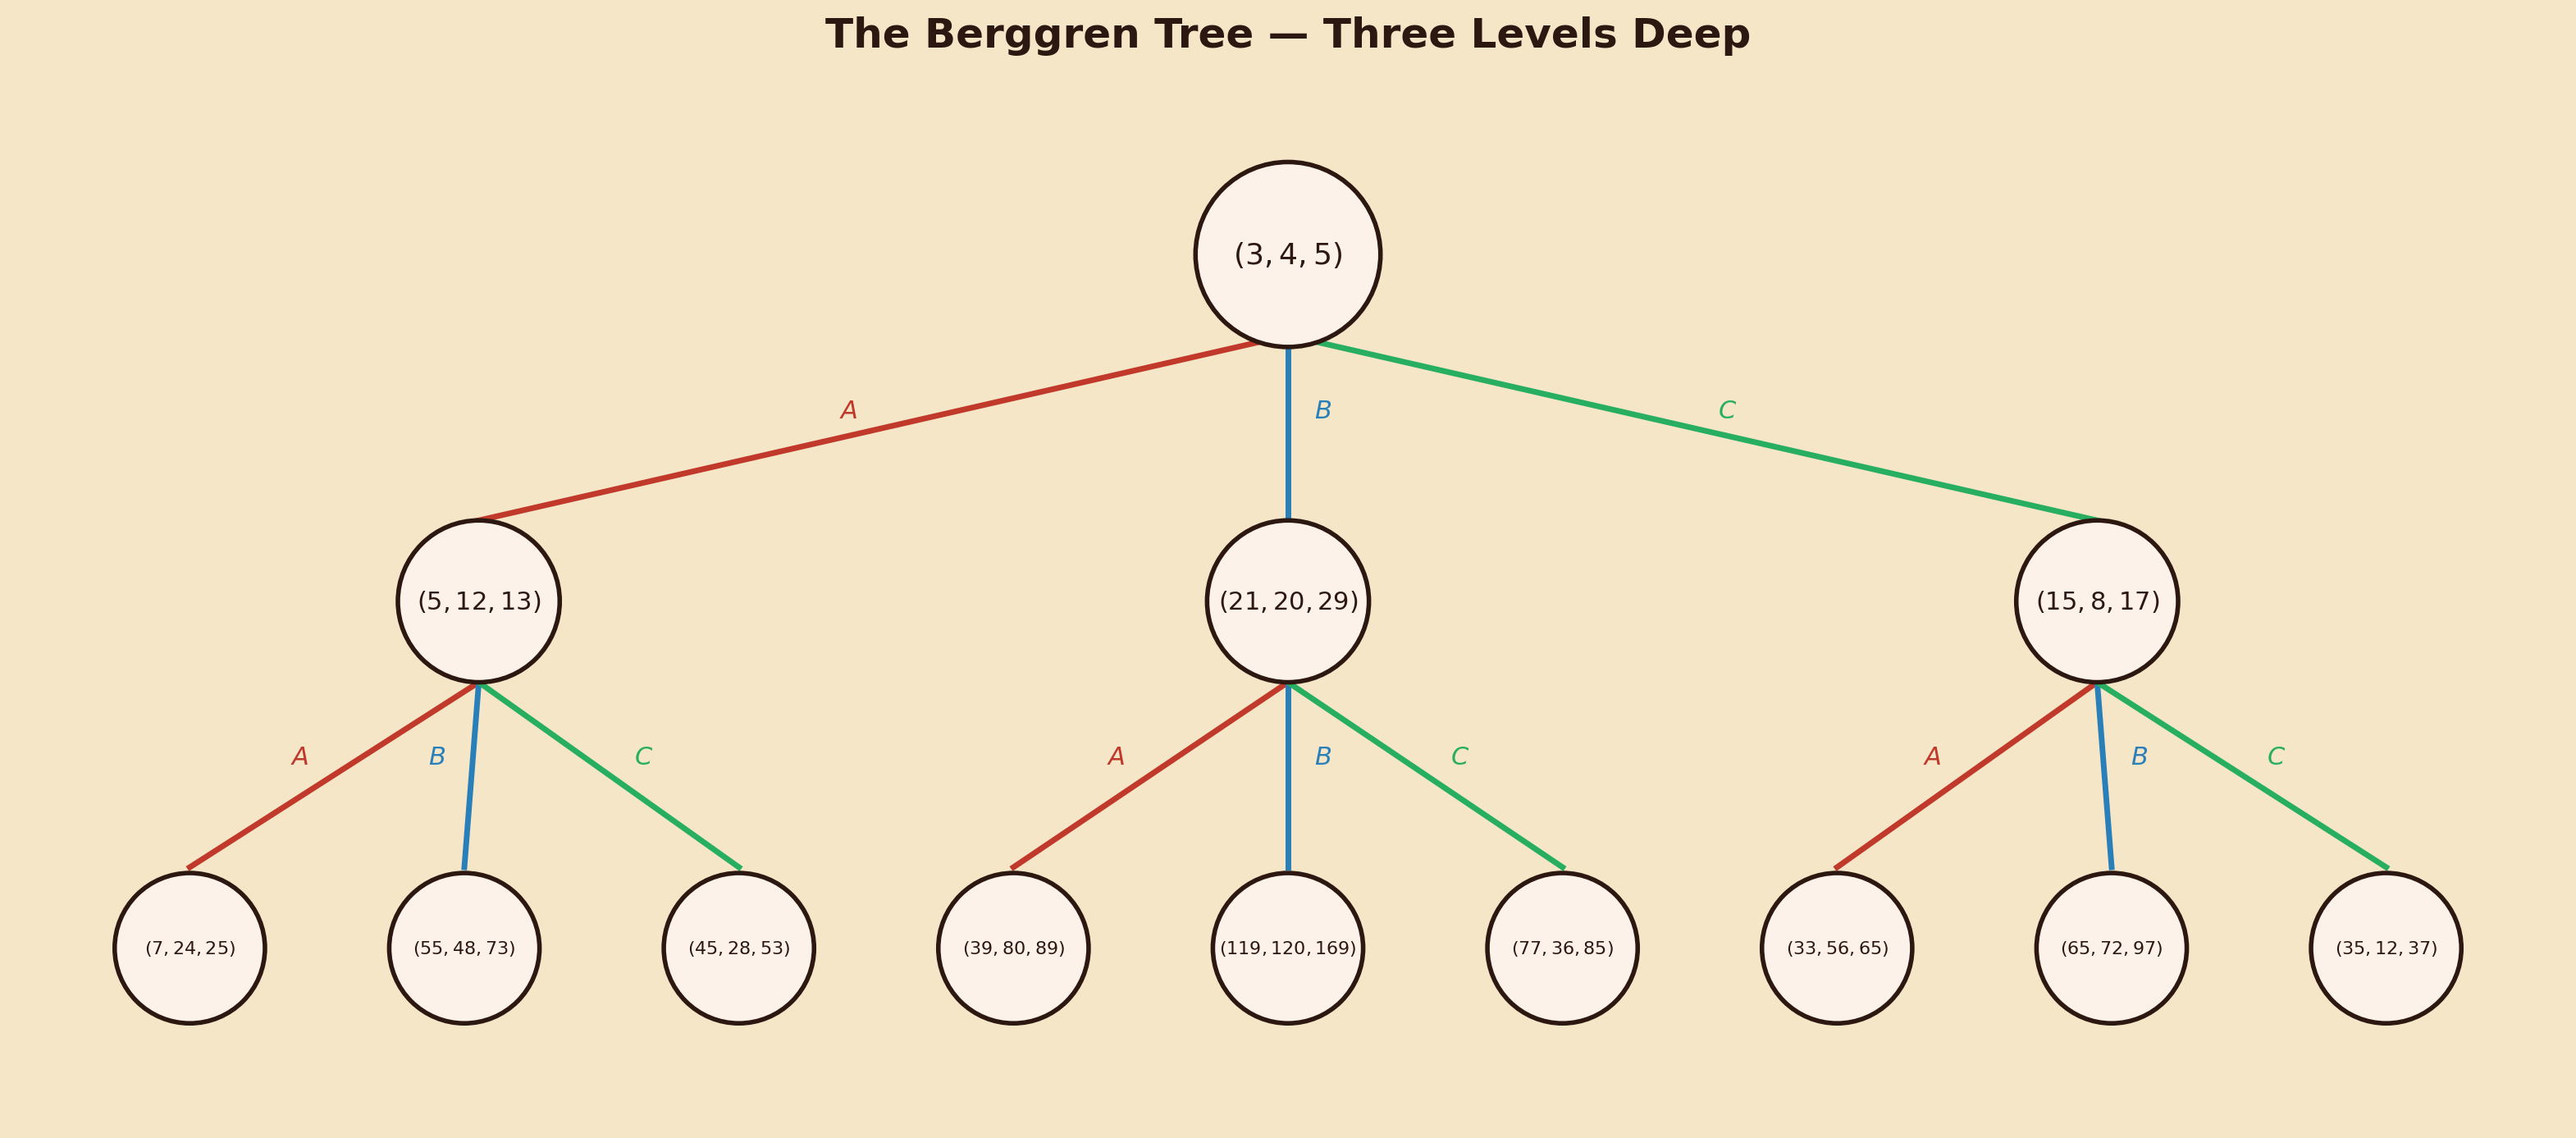
\includegraphics[width=0.85\textwidth]{Chapter5/images/fig01_berggren_tree.png}
\caption{}
\end{figure}
A full ternary tree diagram, three levels deep, rooted at \((3,4,5)\). Each node is a circle containing a Pythagorean triple \((a, b, c)\). The three downward branches from each node are labeled \(A\), \(B\), \(C\). At the first level: \((5,12,13)\), \((21,20,29)\), \((15,8,17)\). At the second level, nine nodes showing the grandchildren. The tree has an organic, fractal appearance --- like a deciduous tree in winter --- with branches spreading wider at each level. At least 13 nodes are visible.{]}


\begin{figure}[htbp]
\centering
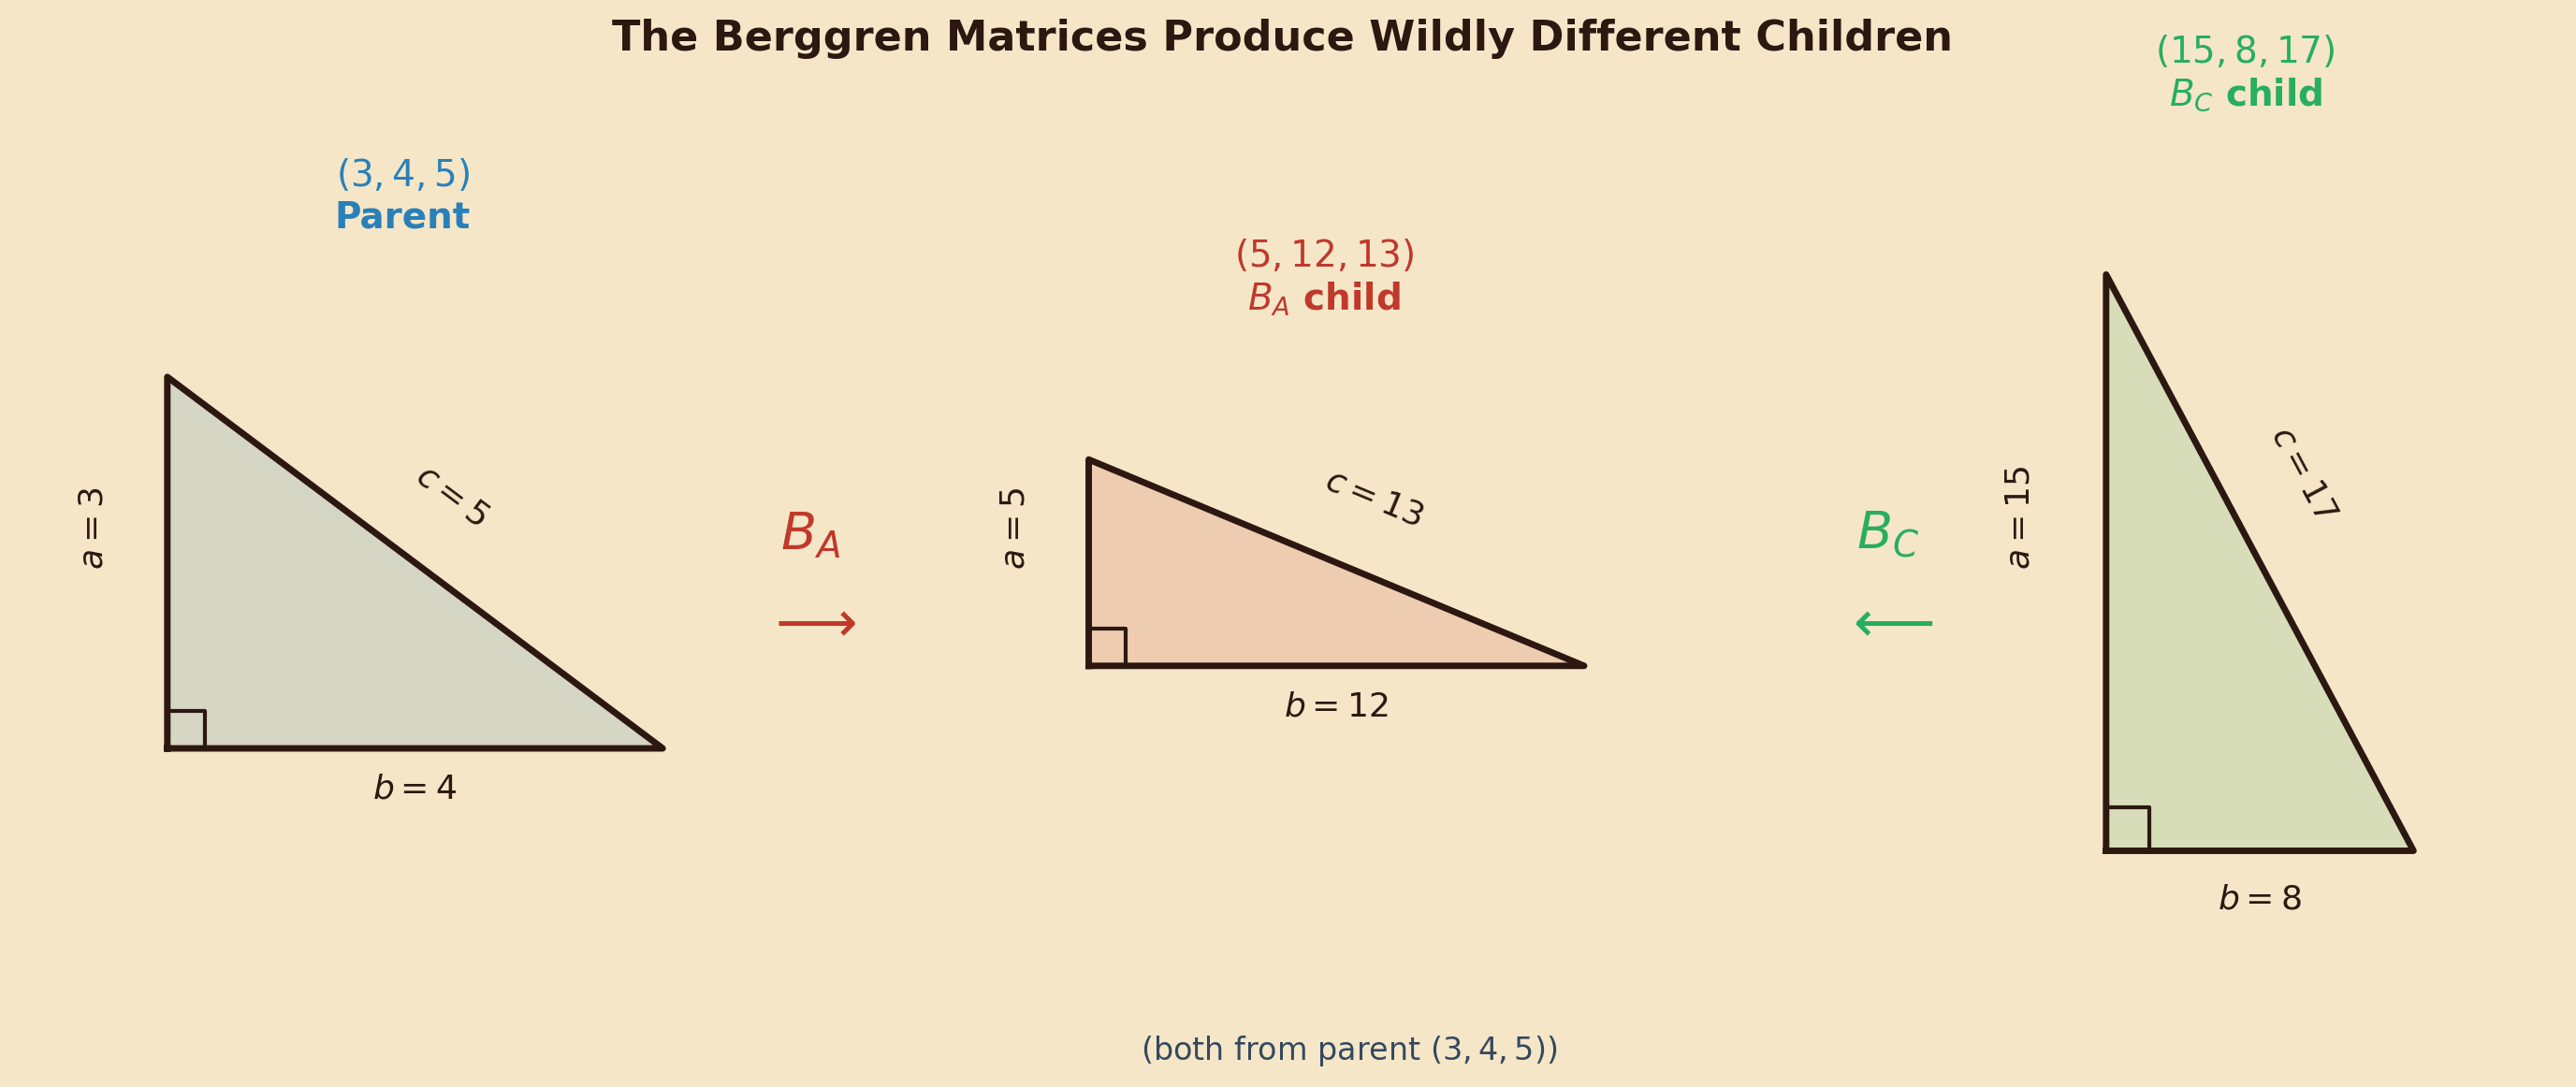
\includegraphics[width=0.85\textwidth]{Chapter5/images/fig02_three_triangles.png}
\caption{}
\end{figure}
Three right triangles drawn to scale: \((3,4,5)\), \((5,12,13)\), and \((15,8,17)\). Each triangle's sides are clearly labeled with lengths. Arrows indicate which Berggren matrix maps one triangle to the next: an arrow from \((3,4,5)\) to \((5,12,13)\) labeled ``\(B_A\)'', and from \((3,4,5)\) to \((15,8,17)\) labeled ``\(B_C\).'' The visual emphasis is on how different the children look --- the matrices produce wildly varied shapes from a single parent.{]}

Berggren published his result in a Swedish journal so obscure that the wider mathematical world took no notice for nearly three decades. His proof was entirely elementary --- matrix arithmetic and a bit of number theory --- yet it achieved something remarkable: a complete, constructive enumeration of an infinite set. As we saw in Chapter 2, the same tree has a twin formulation in the \(2 \times 2\) world of Euclid's parameters \((m, n)\). But the \(3 \times 3\) formulation, acting directly on triples, is the one that will reveal the deeper geometry.

That deeper geometry is the subject of this chapter. The three Berggren matrices are not arbitrary. They are not the result of trial and error or divine inspiration. They are elements of a specific algebraic structure --- one that governs the geometry of Einstein's spacetime. The tree of Pythagorean triples, it turns out, is a discrete tiling of hyperbolic space. Its branches are the integer symmetries of a light cone.

But I am getting ahead of the story. Let us begin with a quantity that seems to care nothing about Pythagoras.

\bigskip\noindent\rule{\linewidth}{0.4pt}\bigskip

\section{The Signature That Doesn't Change}
Here is a puzzle within a puzzle. Take \emph{any} triple of integers \((a, b, c)\) --- Pythagorean or not --- and compute

\[Q(a, b, c) = a^2 + b^2 - c^2.\]

We have already met \(Q\) in Chapter 1: for Pythagorean triples, \(Q = 0\), and that is what it means to be Pythagorean. But now I want you to watch what happens when you apply a Berggren matrix to a triple that is \emph{not} on the null cone --- say \((1, 2, 3)\), for which \(Q(1, 2, 3) = 1 + 4 - 9 = -4\).

Multiply: \(B_A \begin{pmatrix} 1 \\ 2 \\ 3 \end{pmatrix} = \begin{pmatrix} 1 - 4 + 6 \\ 2 - 2 + 6 \\ 2 - 4 + 9 \end{pmatrix} = \begin{pmatrix} 3 \\ 6 \\ 7 \end{pmatrix}.\) Now compute \(Q(3, 6, 7) = 9 + 36 - 49 = -4.\) The same value! Try \(B_B\) and \(B_C\) on the same input --- you will get \(-4\) every time.

This is no coincidence. It is the central fact of this chapter, and it deserves a careful statement.

\textbf{Theorem (Lorentz Form Preservation).} Let \(\eta\) denote the diagonal matrix

\[\eta = \begin{pmatrix} 1 & 0 & 0 \\ 0 & 1 & 0 \\ 0 & 0 & -1 \end{pmatrix},\]

so that \(Q(\mathbf{v}) = \mathbf{v}^\top \eta\, \mathbf{v}\). Then for each \(M \in \{B_A, B_B, B_C\}\),

\[M^{\!\top}\, \eta\, M = \eta.\]

This equation says that every Berggren matrix preserves the quadratic form \(Q\) --- not just on the null cone, not just for Pythagorean triples, but for \emph{every} integer vector in \(\mathbb{Z}^3\). For any \(\mathbf{v}\),

\[Q(M\mathbf{v}) = (M\mathbf{v})^\top \eta\, (M\mathbf{v}) = \mathbf{v}^\top M^\top \eta\, M\, \mathbf{v} = \mathbf{v}^\top \eta\, \mathbf{v} = Q(\mathbf{v}).\]

The proof of the theorem is direct computation. Let me walk through the case \(M = B_A\) in detail, so you can see the machinery (and verify it yourself on the back of an envelope). We need to show that for arbitrary integers \(a, b, c\):

\[Q(a - 2b + 2c,\; 2a - b + 2c,\; 2a - 2b + 3c) = Q(a, b, c).\]

Expand the left-hand side. The first component squared is

\[(a - 2b + 2c)^2 = a^2 + 4b^2 + 4c^2 - 4ab + 4ac - 8bc.\]

The second component squared is

\[(2a - b + 2c)^2 = 4a^2 + b^2 + 4c^2 - 4ab + 8ac - 4bc.\]

The third component squared is

\[(2a - 2b + 3c)^2 = 4a^2 + 4b^2 + 9c^2 - 8ab + 12ac - 12bc.\]

Add the first two and subtract the third:

\[(a^2 + 4b^2 + 4c^2 - 4ab + 4ac - 8bc) + (4a^2 + b^2 + 4c^2 - 4ab + 8ac - 4bc) - (4a^2 + 4b^2 + 9c^2 - 8ab + 12ac - 12bc).\]

Collect terms: - \(a^2\): \(1 + 4 - 4 = 1\). - \(b^2\): \(4 + 1 - 4 = 1\). - \(c^2\): \(4 + 4 - 9 = -1\). - \(ab\): \(-4 - 4 + 8 = 0\). - \(ac\): \(4 + 8 - 12 = 0\). - \(bc\): \(-8 - 4 + 12 = 0\).

The result is \(a^2 + b^2 - c^2 = Q(a, b, c)\). Every cross-term cancels perfectly --- a small algebraic miracle that is, in fact, not a miracle at all, but the fingerprint of a symmetry group.

The cases \(B_B\) and \(B_C\) work out identically. The computations are the same in character, if slightly different in sign; I invite you to verify one of them for the pleasure of watching the cancellation unfold.

Now: what \emph{is} a matrix that satisfies \(M^\top \eta\, M = \eta\)? In the language of physics, it is a \textbf{Lorentz transformation} --- the very same class of transformations that Hermann Minkowski, Hendrik Lorentz, and Albert Einstein used to describe the symmetries of spacetime. The matrix \(\eta\) is the \textbf{Minkowski metric}, the ``ruler'' of special relativity, which measures the interval between events using that famous minus sign in the time coordinate. A Lorentz transformation is any linear map that preserves this ruler --- that leaves the spacetime interval unchanged.

The collection of all such matrices forms a group, denoted \(O(2, 1)\): the orthogonal group of a quadratic form with two positive signs and one negative sign. Our Berggren matrices live in the subgroup \(O(2, 1; \mathbb{Z})\) --- the \emph{integer} Lorentz group, whose entries are restricted to whole numbers. This is a discrete, countable subgroup of a continuous family, and it is exactly the right structure for enumerating lattice points on a cone.


\begin{figure}[htbp]
\centering

\includegraphics[width=0.85\textwidth]{Chapter5/images/fig03_null_cone.png}
\caption{}
\end{figure}
A three-dimensional coordinate system with axes labeled \(a\), \(b\), \(c\). A cone (the ``light cone'') is drawn satisfying \(a^2 + b^2 = c^2\), i.e., \(Q = 0\). The cone opens upward along the \(c\)-axis. Several Pythagorean triples are plotted as bright glowing dots on the cone's surface: \((3,4,5)\), \((5,12,13)\), \((8,15,17)\), \((7,24,25)\). The cone is rendered semi-transparently, revealing the lattice of integer points inside and outside it. Caption: ``The null cone of \(Q\): every Pythagorean triple lives here.''{]}


\begin{figure}[htbp]
\centering
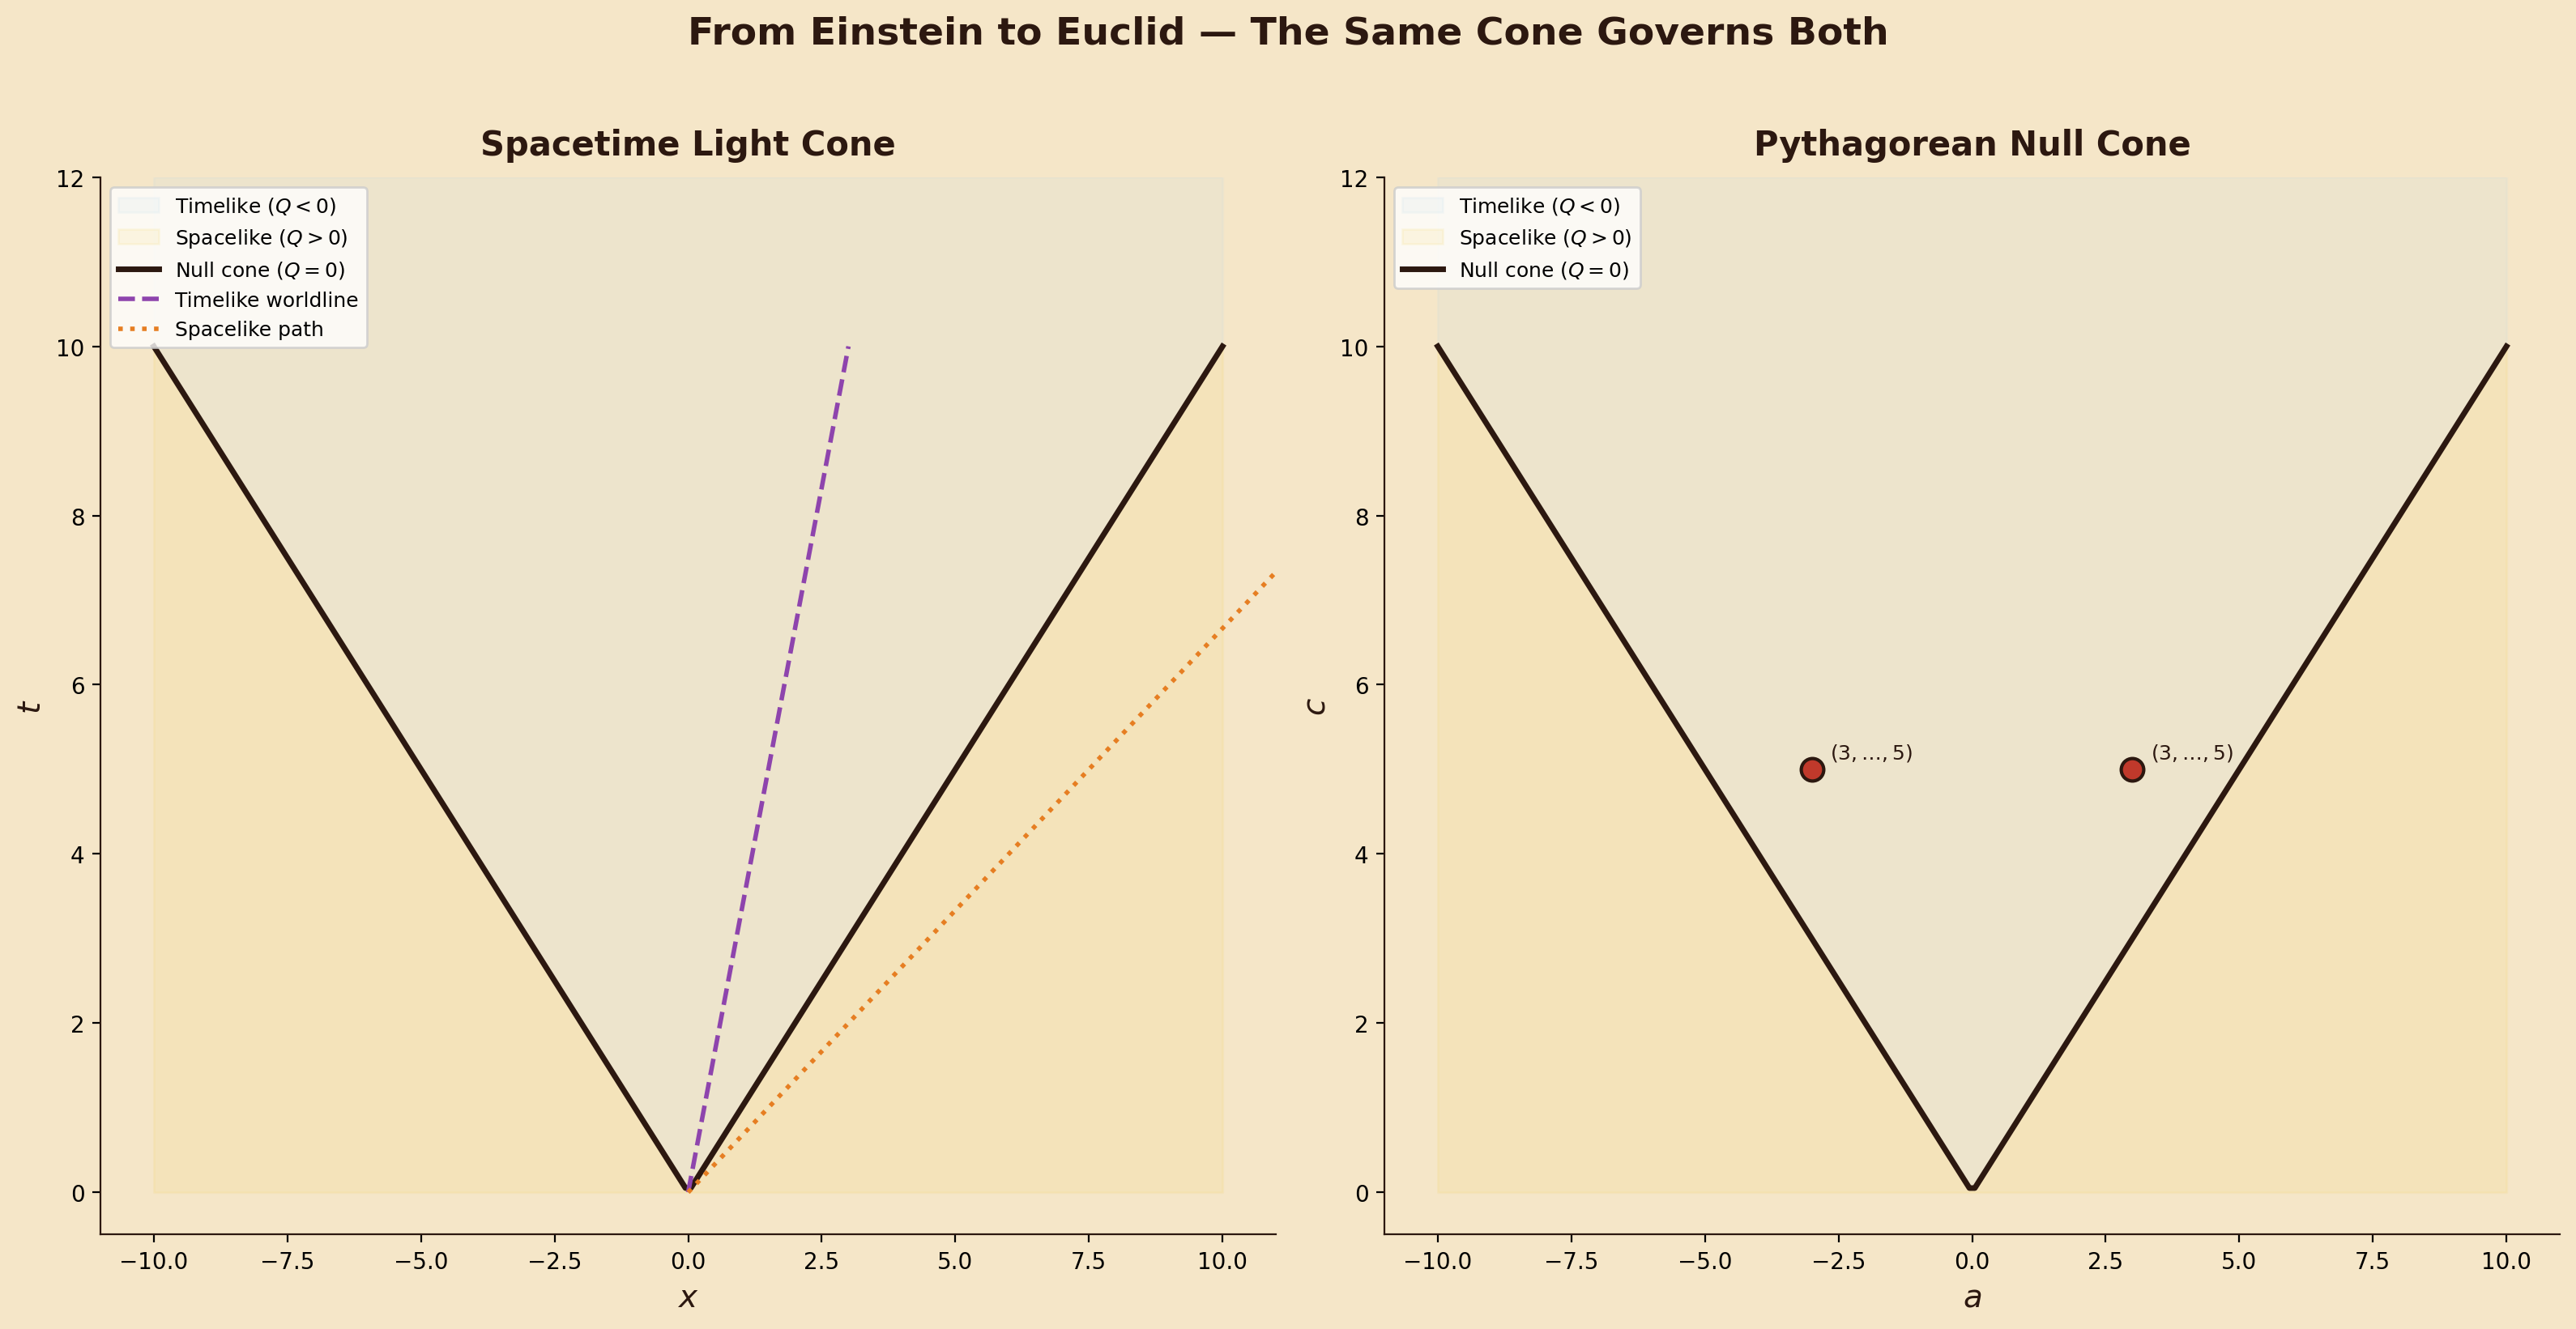
\includegraphics[width=0.85\textwidth]{Chapter5/images/fig04_spacetime_comparison.png}
\caption{}
\end{figure}
Side-by-side comparison. LEFT: A classic spacetime diagram from physics, showing a light cone with two worldlines --- one timelike (inside the cone) and one spacelike (outside). The axes are labeled \(x\), \(y\), \(t\). RIGHT: The same cone but with axes \(a\), \(b\), \(c\), populated with Pythagorean triples as labeled dots. The visual punchline: they are the \emph{same} mathematical object. Caption: ``From Einstein to Euclid --- the same cone governs both.''{]}

The coincidence is stunning, and it is not superficial. The reason the Berggren matrices generate all primitive Pythagorean triples is precisely \emph{because} they generate (a subgroup of) the integer Lorentz group. The integer points on the null cone are permuted by Lorentz transformations --- just as the rational points on a circle are permuted by rotations --- and the Berggren matrices happen to act transitively on the primitive ones. The tree is not a trick; it is a consequence of the symmetry of spacetime geometry.

\bigskip\noindent\rule{\linewidth}{0.4pt}\bigskip

\section{Orientation --- The Subtle Art of the Determinant}
Two of our three matrices are right-handed. One is left-handed. Can you tell which, just by looking?

Compute the determinants:

\[\det(B_A) = 1, \qquad \det(B_B) = -1, \qquad \det(B_C) = 1.\]

I will spare you the full cofactor expansion --- it is a standard exercise --- but you can spot the answer quickly by noting that \(B_B\) is the only matrix with all positive entries. The negative entries in \(B_A\) and \(B_C\) collaborate to produce positive determinants; the relentless positivity of \(B_B\) tips the balance the other way. Mathematics is occasionally ironic.

What does a determinant of \(\pm 1\) mean geometrically? A matrix with determinant \(+1\) is a \emph{proper} transformation --- a rotation of the underlying space (here, hyperbolic space). A matrix with determinant \(-1\) includes a reflection: it flips the orientation, like looking in a mirror. Both types belong to the full Lorentz group \(O(2, 1; \mathbb{Z})\), but the proper transformations form a special subgroup, \(SO(2, 1; \mathbb{Z})\), the ``S'' standing for ``special'' (determinant one). Our matrices \(B_A\) and \(B_C\) live in this special subgroup; \(B_B\) does not.

This distinction has a subtle but beautiful consequence for the tree. Every time you follow the \(B\)-branch, you introduce a mirror flip. Follow it twice: two flips compose to the identity, and you are back to a proper rotation. Follow it three times: a flip again. The \(B\)-branch oscillates between rotations and reflections like a pendulum swinging between left and right.

Here is a small puzzle to test your understanding: \emph{If you follow the \(B\)-branch for ten steps --- that is, apply \(B_B\) ten times in succession --- is the resulting transformation a rotation or a reflection?} The answer is immediate: \(\det(B_B^{10}) = (-1)^{10} = 1\), so it is a rotation. An even number of reflections always composes to a rotation; an odd number gives a reflection. This is the algebraic manifestation of a fact every child discovers with two hand mirrors: an even number of reflections returns you to the ``right way round.''


\begin{figure}[htbp]
\centering
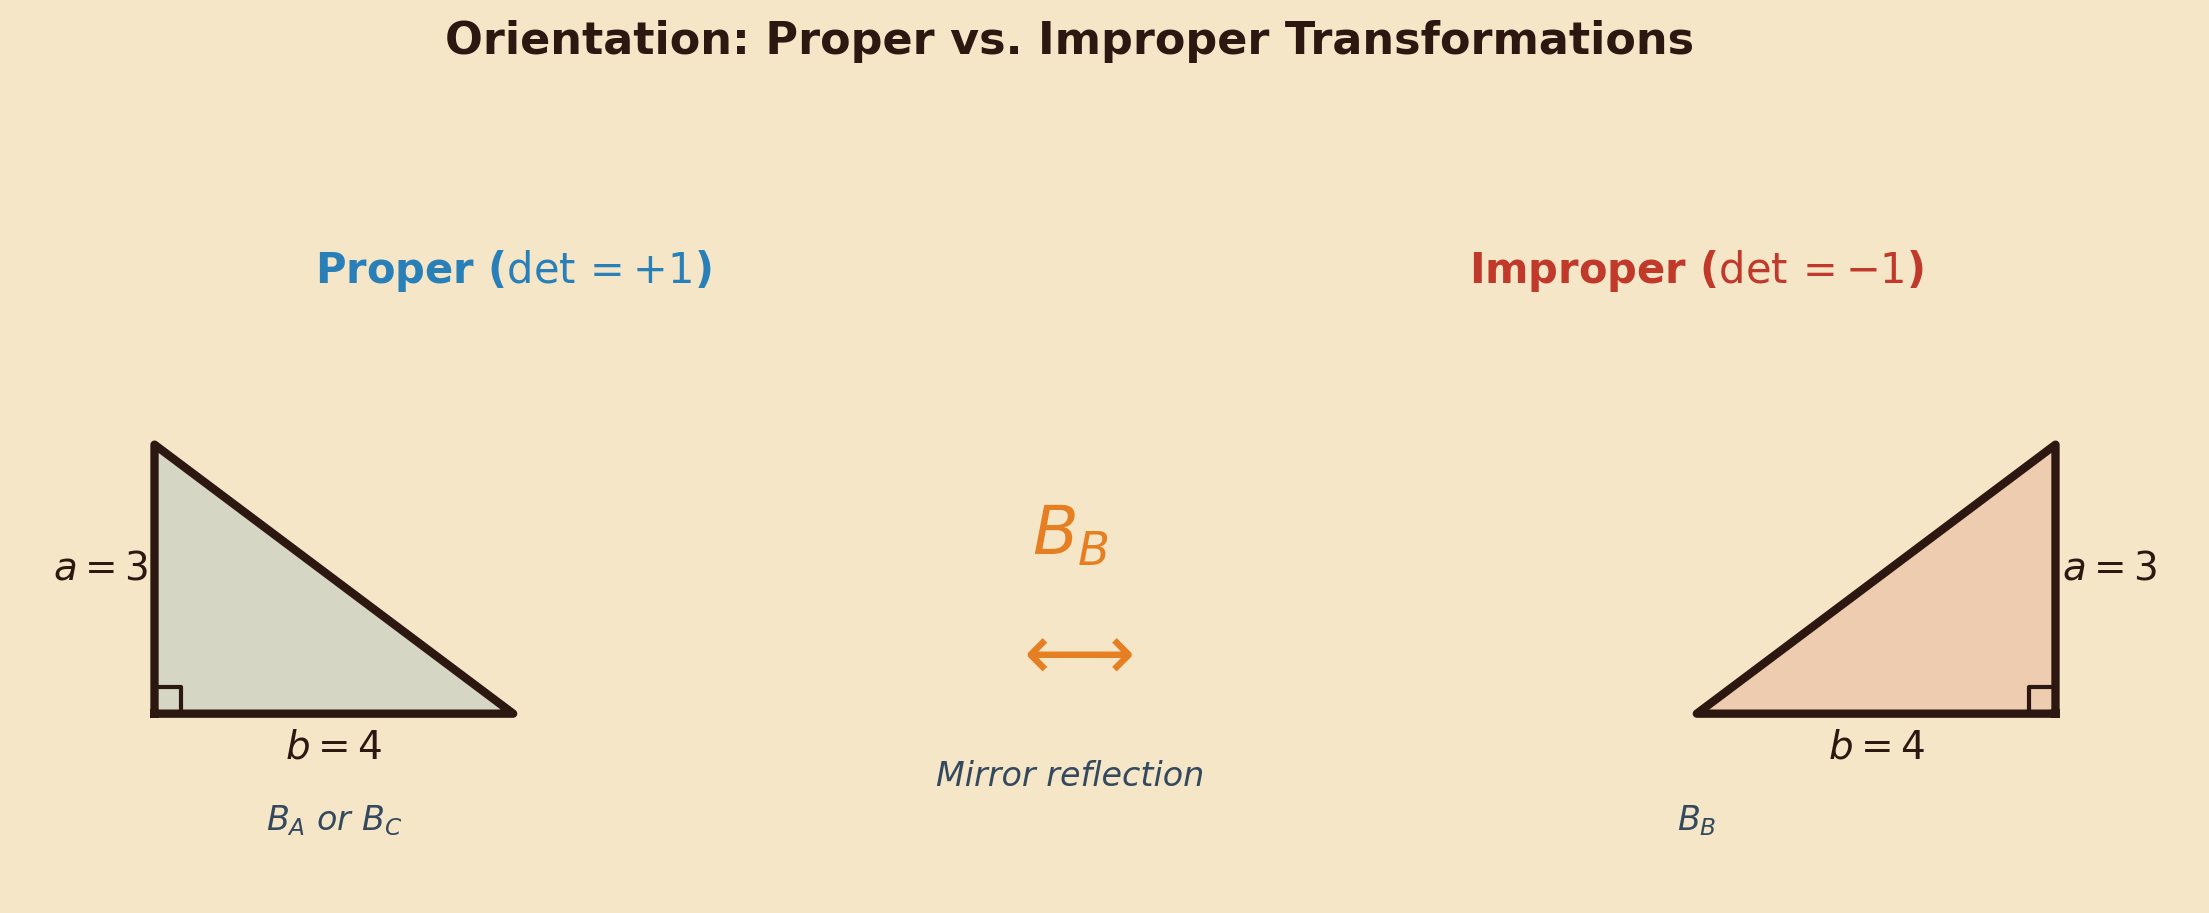
\includegraphics[width=0.85\textwidth]{Chapter5/images/fig05_mirror_triangle.png}
\caption{}
\end{figure}
Two versions of a right triangle \((3,4,5)\), one the mirror image of the other (reflected across a vertical axis). The left triangle is labeled ``proper'' (\(\det = +1\)), the right is labeled ``improper'' (\(\det = -1\)). A curved arrow between them is labeled ``\(B_B\).'' The visual metaphor: the triangle is flipped as if viewed in a mirror. A second curved arrow returns from right to left, labeled ``\(B_B\) again,'' with the note ``\((-1)^2 = +1\).''{]}

The \(A\)- and \(C\)-branches, by contrast, are always proper. They rotate without flipping. The full tree is thus a mix of two flavors of transformation: the \(A\)- and \(C\)-branches preserve handedness; the \(B\)-branch reverses it. This asymmetry is invisible if you look only at the triples --- a Pythagorean triple has no ``handedness'' --- but it is visible in the algebraic structure of the paths from root to leaf.

\bigskip\noindent\rule{\linewidth}{0.4pt}\bigskip

\section{Why Every Child Is Pythagorean}
It is one thing to check that \((5, 12, 13)\) satisfies \(a^2 + b^2 = c^2\). It is another thing entirely to \emph{know}, without checking, that the triple at the ten-thousandth node --- whichever branching path you took to get there --- must also be Pythagorean. Here is why you can be certain.

\textbf{Theorem (Pythagorean Preservation).} If \(a^2 + b^2 = c^2\), then each of the three image triples produced by \(B_A\), \(B_B\), and \(B_C\) also satisfies the Pythagorean equation.

Let me state all three explicitly. If \(a^2 + b^2 = c^2\), then:

\[\text{($B_A$): } (a - 2b + 2c)^2 + (2a - b + 2c)^2 = (2a - 2b + 3c)^2,\]

\[\text{($B_B$): } (a + 2b + 2c)^2 + (2a + b + 2c)^2 = (2a + 2b + 3c)^2,\]

\[\text{($B_C$): } (-a + 2b + 2c)^2 + (-2a + b + 2c)^2 = (-2a + 2b + 3c)^2.\]

Each identity is a statement purely about the ring of integers: expand both sides, invoke \(a^2 + b^2 = c^2\) once, and watch the terms collapse. Let me walk through the \(B_A\) case.

The left-hand side is

\[(a - 2b + 2c)^2 + (2a - b + 2c)^2.\]

Expand:

\[= a^2 - 4ab + 4ac + 4b^2 - 8bc + 4c^2 + 4a^2 - 4ab + 8ac + b^2 - 4bc + 4c^2\] \[= 5a^2 + 5b^2 + 8c^2 - 8ab + 12ac - 12bc.\]

The right-hand side is

\[(2a - 2b + 3c)^2 = 4a^2 + 4b^2 + 9c^2 - 8ab + 12ac - 12bc.\]

Subtract: the left exceeds the right by \(a^2 + b^2 - c^2\). But the hypothesis tells us \(a^2 + b^2 - c^2 = 0\), so the two sides are equal. The proof is complete.

Notice the key trick: the difference between the two sides is \emph{exactly} \(Q(a, b, c) = a^2 + b^2 - c^2\). This is no accident --- it is the Lorentz preservation theorem in disguise. Since \(M^\top \eta\, M = \eta\), the form \(Q\) is invariant; and since \(Q = 0\) is the Pythagorean condition, the Pythagorean property is invariant too. The two theorems are logically equivalent.

\textbf{Theorem (Tree Soundness).} Every triple produced by the Berggren tree satisfies \(a^2 + b^2 = c^2\).

The proof is by \textbf{structural induction} --- the tree's own logic turned into a proof technique. The argument has two steps, mirroring the two parts of any inductive proof:

\begin{enumerate}
\def\labelenumi{\arabic{enumi}.}
\tightlist
\item
  \textbf{Base case.} The root is \((3, 4, 5)\). Check: \(9 + 16 = 25\). ✓
\item
  \textbf{Inductive step.} If a node \((a, b, c)\) satisfies \(a^2 + b^2 = c^2\), then by the Pythagorean Preservation theorem, so do its three children.
\end{enumerate}

Therefore every node in the tree --- at depth 1, depth 100, or depth \(10^{10}\) --- is Pythagorean. The property cascades from parent to child like a genetic trait, unfailingly transmitted at every generation.


\begin{figure}[htbp]
\centering
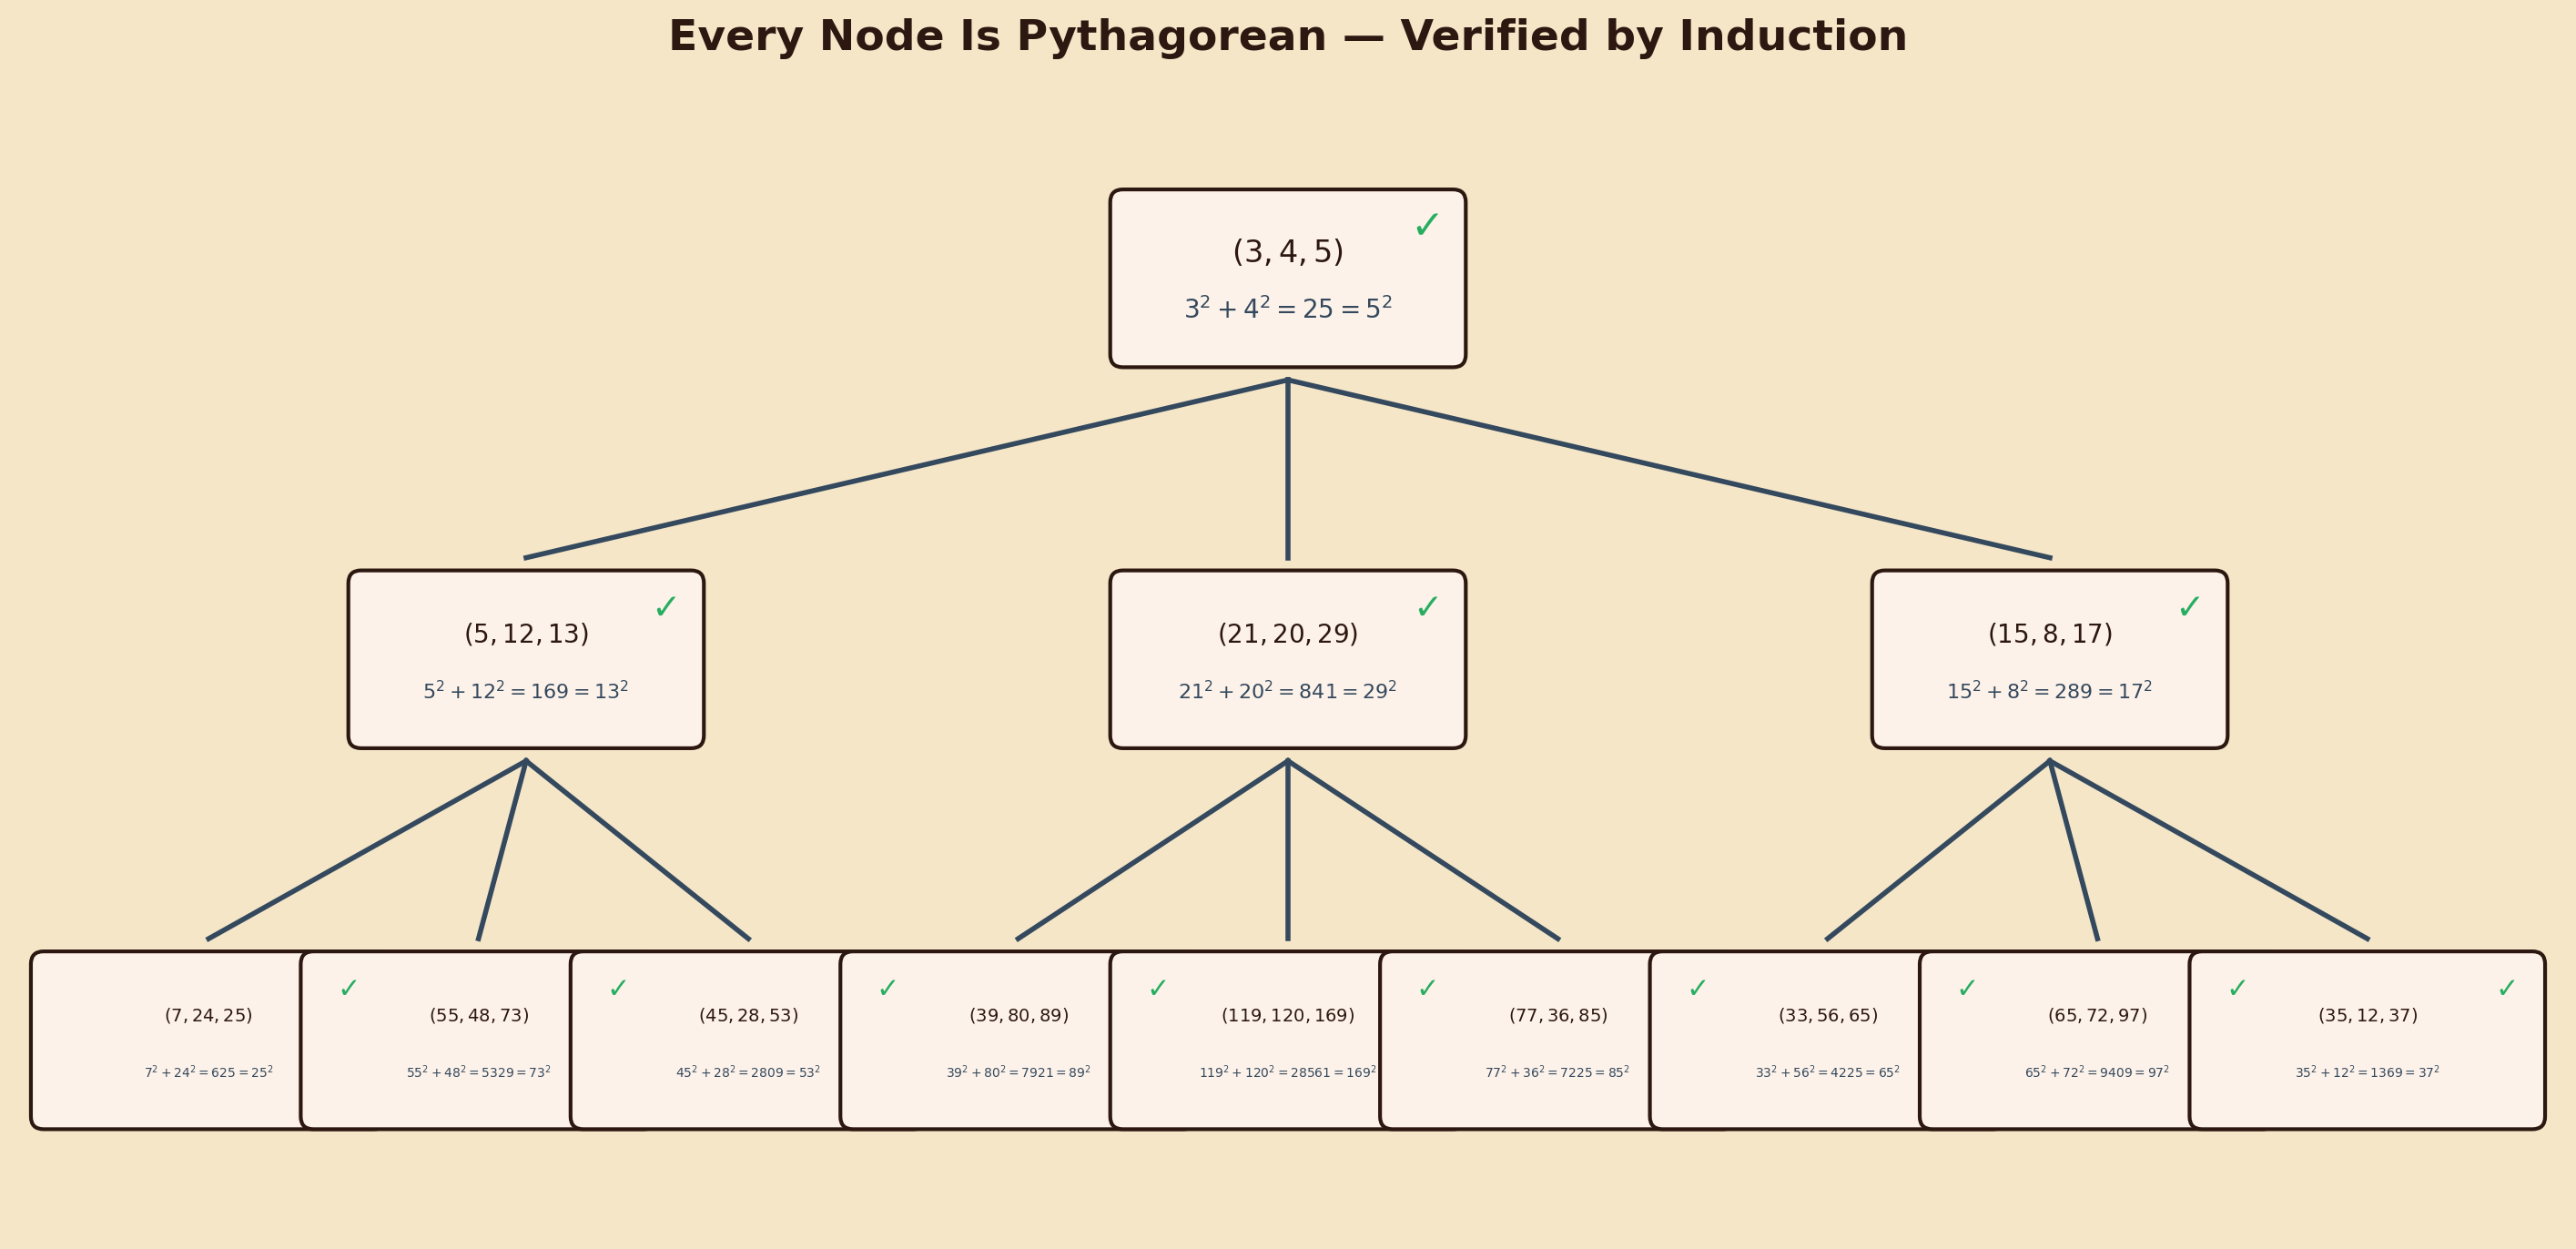
\includegraphics[width=0.85\textwidth]{Chapter5/images/fig06_pythagorean_check.png}
\caption{}
\end{figure}
A segment of the Berggren tree (3 levels deep), with each node's triple displayed inside a circle. Alongside each triple, the values \(a^2 + b^2\) and \(c^2\) are computed explicitly, demonstrating equality. A bold checkmark symbol (✓) appears at each node, rendered in green. The visual message: the Pythagorean property cascades down the tree like a guarantee stamped on every generation.{]}

This is what makes the tree \emph{self-certifying}. You never need to check individual nodes. The proof \emph{is} the structure. It is the mathematical equivalent of heredity: a theorem about \((3, 4, 5)\) becomes a theorem about infinitely many triples, because the tree's branching operations preserve the property that matters.

A brief historical aside: the principle of mathematical induction is usually stated for natural numbers --- prove \(P(0)\), and prove that \(P(n)\) implies \(P(n+1)\), and you have \(P(n)\) for all \(n\). But induction on \emph{trees} (what logicians call ``structural induction'') is a natural and powerful generalization. The idea is ancient --- Pascal used it, Peano axiomatized it --- but the tree version makes the logic feel more vivid. The tree \emph{is} the proof.

\bigskip\noindent\rule{\linewidth}{0.4pt}\bigskip

\section{Living on the Null Cone}
In Einstein's universe, light travels along surfaces where ``distance'' equals zero. Not the Euclidean distance --- that is always positive --- but the \emph{spacetime interval}, the quantity \(x^2 + y^2 - (ct)^2\) where \(c\) is the speed of light (not our hypotenuse, for once). The surfaces where this interval vanishes form a cone in spacetime, and this cone --- the \emph{null cone}, or \emph{light cone} --- is the most important geometric object in all of physics. It separates the events you can influence from the events you cannot.

In the universe of Pythagorean triples, every triple lives on precisely the same kind of surface. The equation \(a^2 + b^2 - c^2 = 0\) defines the null cone of the Lorentz form \(Q\). This is not a metaphor or a loose analogy --- it is exactly the same algebraic condition, the same quadratic form, the same cone. Only the physical interpretation differs.

This observation gives us an alternative, more conceptual proof of tree soundness. Since:

\begin{itemize}
\tightlist
\item
  the Berggren matrices preserve \(Q\) for \emph{all} integer vectors (Lorentz Preservation), and
\item
  the root \((3, 4, 5)\) satisfies \(Q(3, 4, 5) = 9 + 16 - 25 = 0\),
\end{itemize}

every descendant must also satisfy \(Q = 0\):

\[Q(3, 4, 5) = 0 \implies Q(B_M \cdot \mathbf{v}) = Q(\mathbf{v}) = 0\]

for any product of Berggren matrices \(B_M\). The null cone is invariant under the integer Lorentz group; the tree explores the cone's integer points; therefore every node is Pythagorean. It is a one-line proof, given the Lorentz theorem.

What about \emph{non-Pythagorean} triples? The form \(Q\) classifies all integer triples into three families:

\begin{itemize}
\tightlist
\item
  \textbf{Null} (\(Q = 0\)): the Pythagorean triples, living on the cone's surface.
\item
  \textbf{Spacelike} (\(Q > 0\)): triples like \((1, 1, 1)\), where \(Q = 1\). These live \emph{outside} the cone.
\item
  \textbf{Timelike} (\(Q < 0\)): triples like \((1, 1, 2)\), where \(Q = -2\). These live \emph{inside} the cone.
\end{itemize}

The Berggren matrices would faithfully preserve these values too --- a spacelike triple stays spacelike, a timelike triple stays timelike --- but the tree never visits them, because it starts on the cone and the cone is invariant. The tree is a guided tour of one particular surface in a three-dimensional integer universe.


\begin{figure}[htbp]
\centering
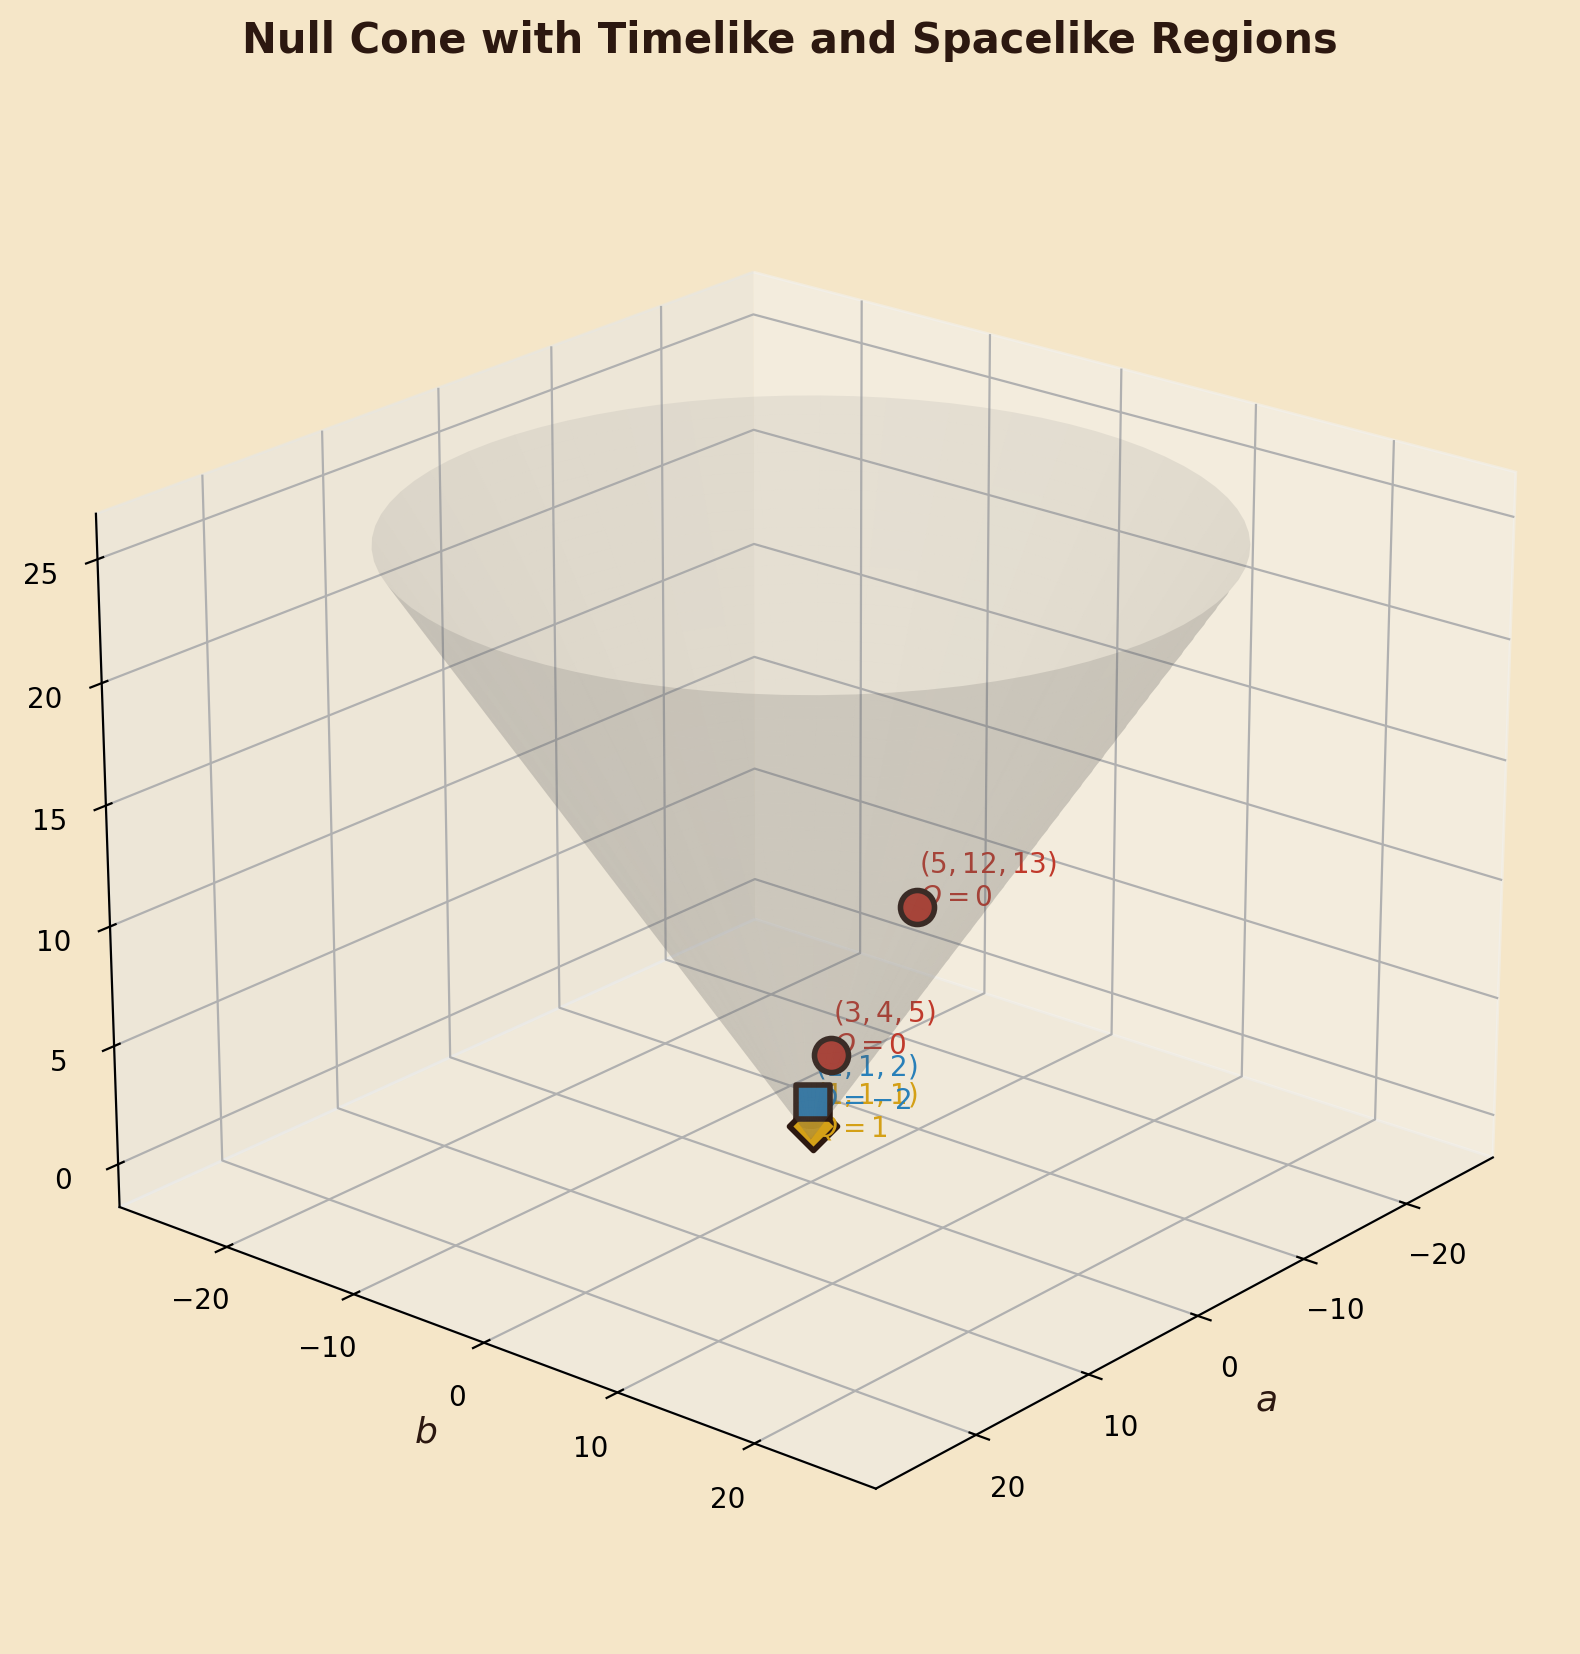
\includegraphics[width=0.85\textwidth]{Chapter5/images/fig07_null_cone_regions.png}
\caption{}
\end{figure}
The null cone \(a^2 + b^2 = c^2\) in 3D, shown with the interior (timelike region, \(Q < 0\)) shaded in cool blue and the exterior (spacelike region, \(Q > 0\)) shaded in warm gold. The cone's surface itself is white or silver. Several labeled points: \((3,4,5)\) and \((5,12,13)\) glowing on the surface; \((1,1,1)\) floating outside in the gold region; \((1,1,2)\) floating inside in the blue region. Each point is annotated with its \(Q\)-value.{]}

Why does the same quadratic form describe both the geometry of light and the arithmetic of right triangles? Is this a coincidence, or a hint at something deeper? I do not have a definitive answer, but I have a suspicion. The form \(Q = x_1^2 + x_2^2 - x_3^2\) is, in a precise algebraic sense, the \emph{simplest} indefinite quadratic form over the integers. It is the first nontrivial object you encounter when you study quadratic forms with mixed signs. Nature, and number theory, both reach for the simplest tools first. That they reach for the \emph{same} tool is perhaps less surprising than it seems --- but no less beautiful for being expected.

\bigskip\noindent\rule{\linewidth}{0.4pt}\bigskip

\section{A Factoring Machine Hidden in the Hypotenuse}
Suppose someone hands you a very large number \(N\) and asks you to find its prime factors. You might reach for a computer, or for the number field sieve, or for Fermat's method. But you might be surprised to learn that a 2,500-year-old theorem about right triangles contains the seed of an answer.

\textbf{Theorem (The Factoring Identity).} For any Pythagorean triple \((a, b, c)\),

\[(c - b)(c + b) = a^2.\]

The proof is one line: \(c^2 - b^2 = a^2\) is just a rearrangement of \(a^2 + b^2 = c^2\). The left-hand side is a difference of squares; the right-hand side is a perfect square. Elementary, yes --- but the implications are anything but.

Think of it this way. If \(N\) is a number you want to factor, and you can find integers \(b\) and \(c\) with \(N^2 + b^2 = c^2\) --- that is, a Pythagorean triple with \(a = N\) --- then you have

\[N^2 = (c - b)(c + b),\]

and the two ``jaws'' \(c - b\) and \(c + b\) squeeze \(N^2\) into a nontrivial factorization. If you are lucky, \(\gcd(N, c - b)\) is a proper factor of \(N\).

This is essentially Fermat's method of factoring, dressed in Pythagorean clothing. Fermat himself would have approved of the presentation, if not the clothing. (He was, after all, a man who preferred to work in the margins.)

The factoring identity is closely related to a much deeper result, one that connects the multiplicative structure of the integers to the geometry of the complex plane.

\textbf{Theorem (The Brahmagupta--Fibonacci Identity).} For any integers \(a_1, b_1, a_2, b_2\),

\[(a_1^2 + b_1^2)(a_2^2 + b_2^2) = (a_1 a_2 - b_1 b_2)^2 + (a_1 b_2 + b_1 a_2)^2.\]

This identity says that the product of two sums of two squares is again a sum of two squares. It is not obvious --- try to see it without the formula, and you will struggle --- but once written down, it is pure algebra: expand both sides and watch the cross-terms vanish.

The identity has a luminous interpretation in the language of Gaussian integers. If \(z_1 = a_1 + b_1 i\) and \(z_2 = a_2 + b_2 i\), then \(|z_1|^2 = a_1^2 + b_1^2\) and \(|z_2|^2 = a_2^2 + b_2^2\), and the identity is simply the statement \(|z_1 z_2|^2 = |z_1|^2 |z_2|^2\) --- the multiplicativity of the complex modulus. This is why the sums of two squares form a \emph{multiplicative} set: the Gaussian integers hand you the bookkeeping for free.

Brahmagupta discovered this identity in India around 628 CE, in his astronomical treatise \emph{Brāhmasphuṭasiddhānta}. Fibonacci rediscovered it in 1225 in his \emph{Liber Quadratorum}. It later became a crucial ingredient in the proof of Fermat's theorem that every prime of the form \(4k + 1\) is a sum of two squares --- a theorem that Fermat stated, characteristically, without proof, and that Euler finally proved a century later after years of effort.

The connection to our factoring identity is this: if \(N^2\) can be written as a sum of two squares in \emph{two different ways}, each representation gives a different pair \((c - b, c + b)\), and comparing these pairs often exposes a factor of \(N\). The more representations you find, the more chances you have. The Brahmagupta--Fibonacci identity is the engine that manufactures these representations by multiplying smaller ones together.


\begin{figure}[htbp]
\centering
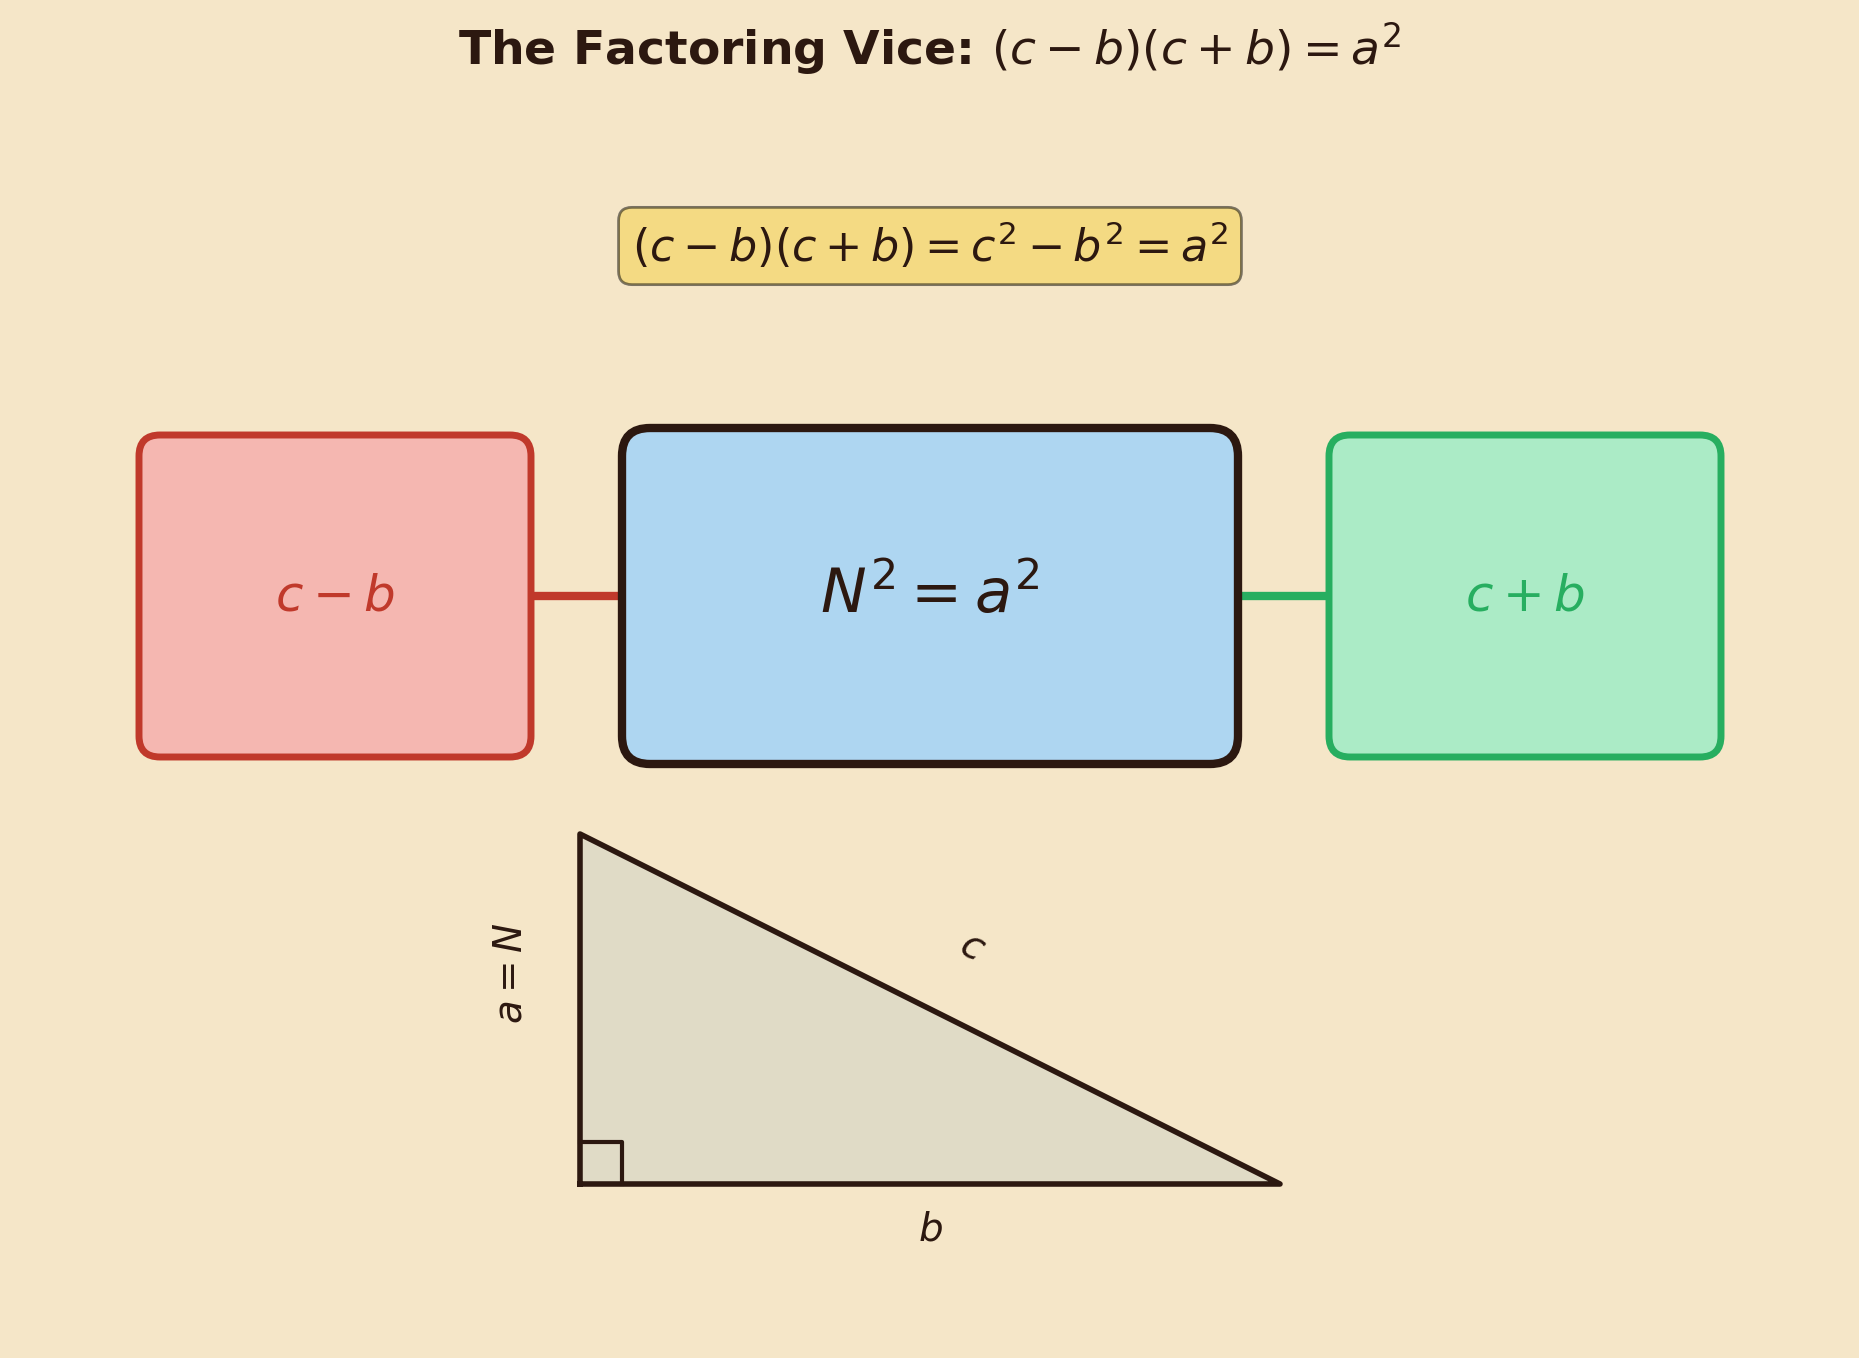
\includegraphics[width=0.85\textwidth]{Chapter5/images/fig08_factoring_vice.png}
\caption{}
\end{figure}
A ``factoring vice'' diagram. A large number \(N^2\) sits in the center, rendered as a heavy block. Two arrows labeled \(c - b\) and \(c + b\) press in from both sides like the jaws of a vice, splitting the block into two factors. Below, a right triangle with hypotenuse \(c\), one leg \(b\), and the other leg \(a = N\), showing the geometric origin of the factorization.{]}


\begin{figure}[htbp]
\centering
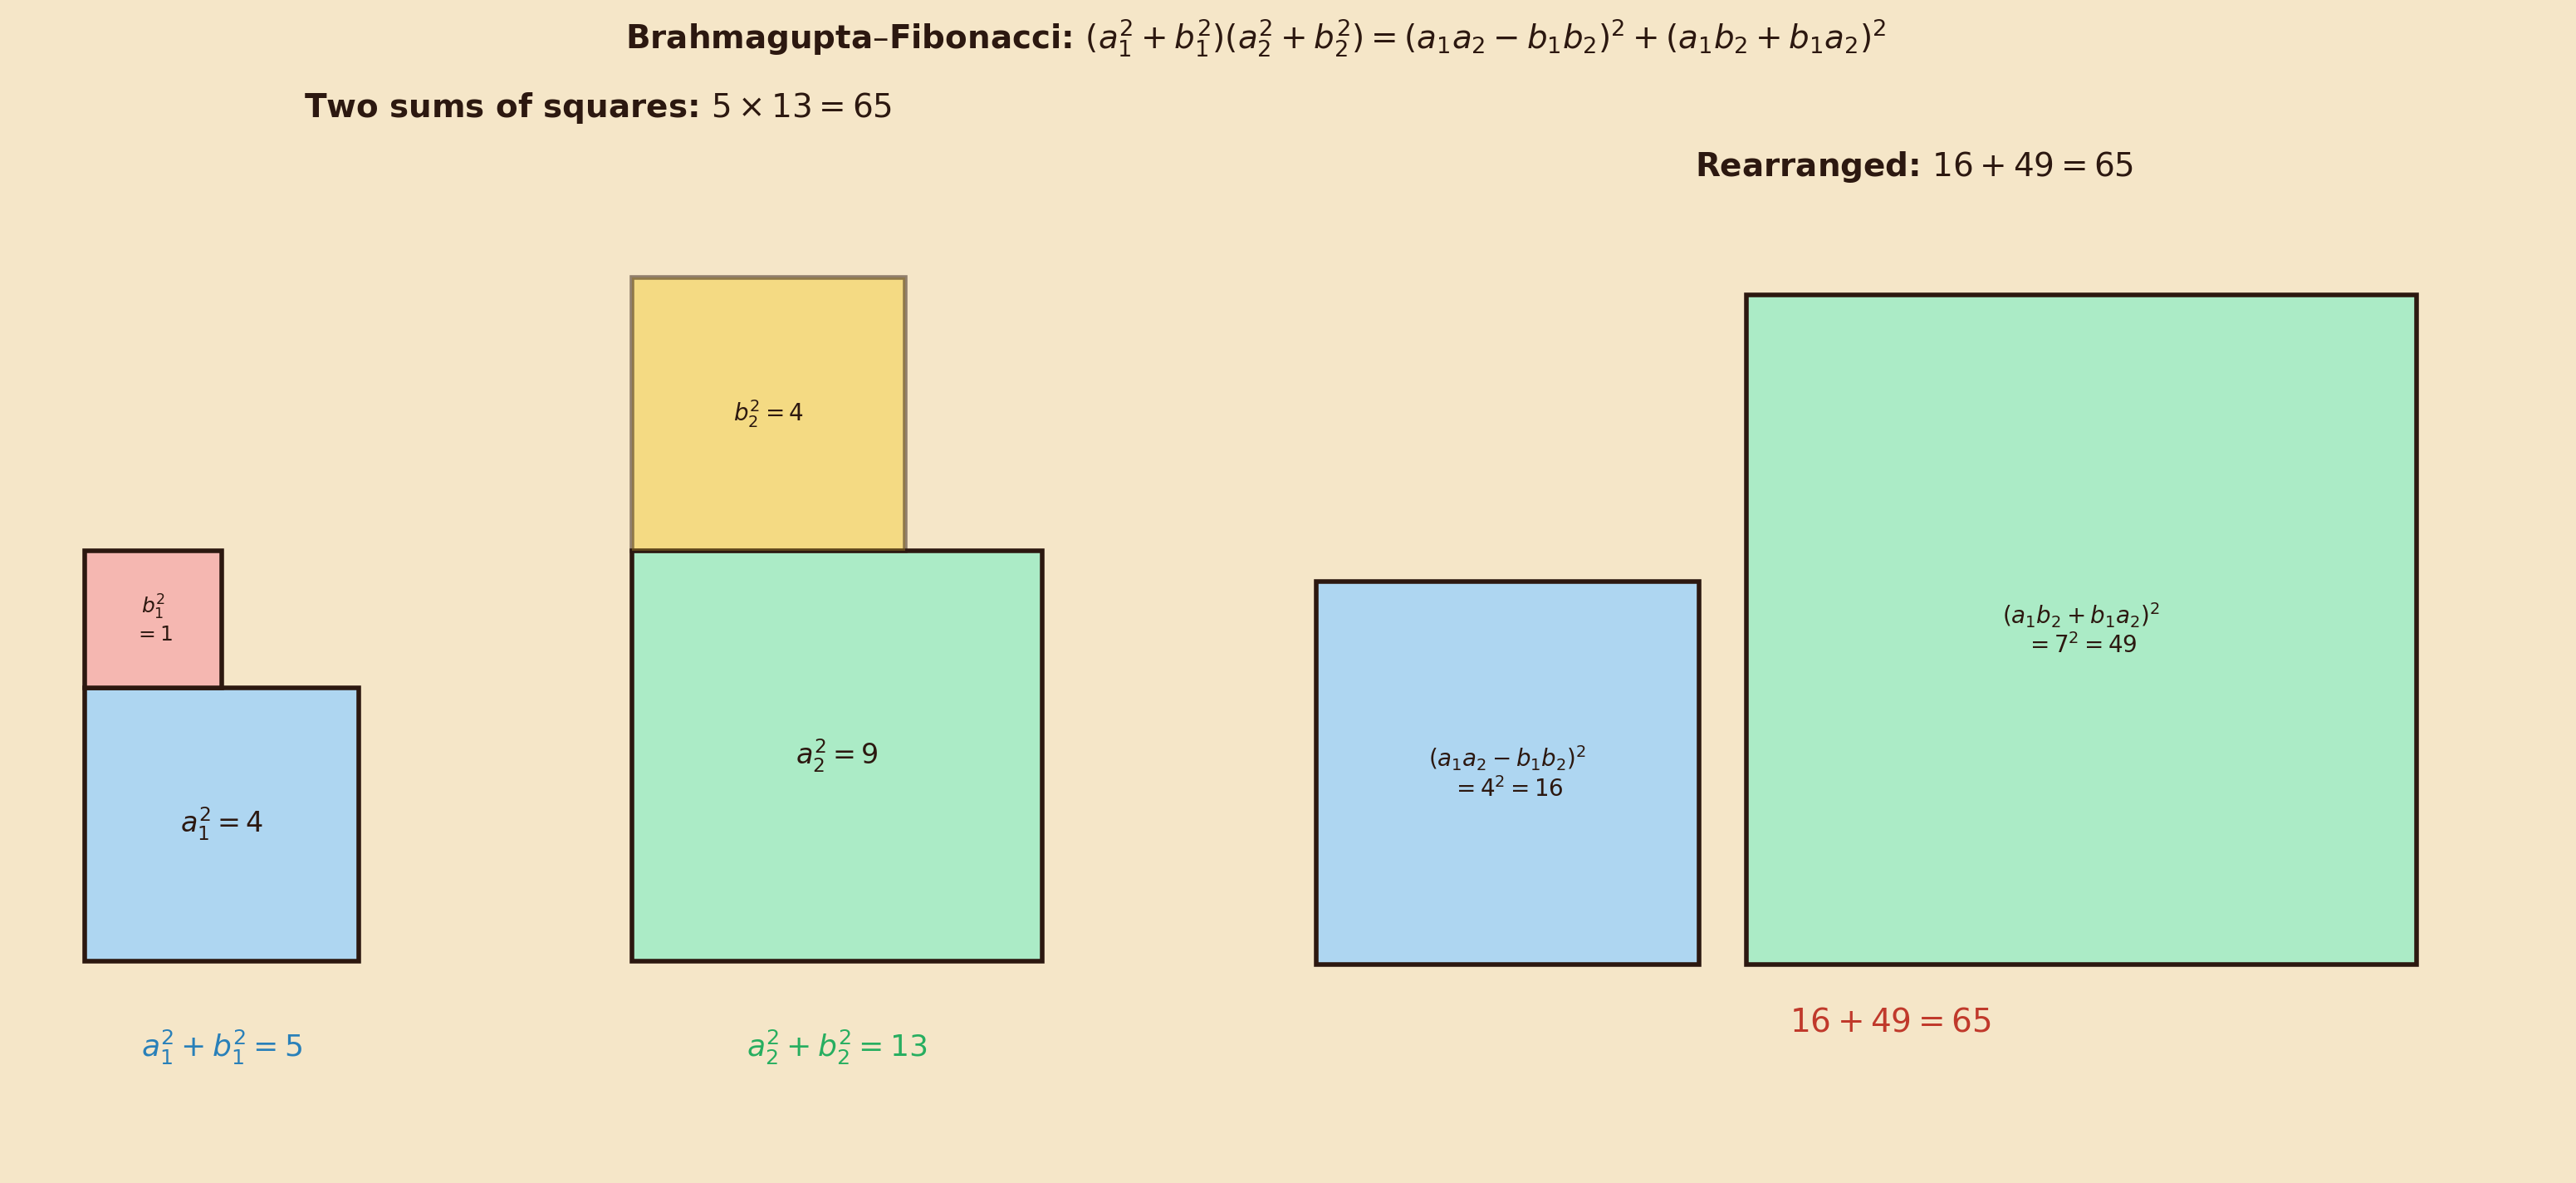
\includegraphics[width=0.85\textwidth]{Chapter5/images/fig09_brahmagupta_fibonacci.png}
\caption{}
\end{figure}
A visual proof of the Brahmagupta--Fibonacci identity using a rectangle subdivided into squares. A large rectangle has area \((a_1^2 + b_1^2)(a_2^2 + b_2^2)\). Through a clever geometric rearrangement --- rotating an inner rectangle --- it is shown to equal \((a_1 a_2 - b_1 b_2)^2 + (a_1 b_2 + b_1 a_2)^2\). The rearrangement is shown step-by-step with colored regions.{]}

\bigskip\noindent\rule{\linewidth}{0.4pt}\bigskip

\section{Euclid's Master Formula}
Every schoolchild knows the triple \((3, 4, 5)\). Fewer know \((5, 12, 13)\) or \((8, 15, 17)\). But Euclid knew a single formula that produces them all --- and its proof is one line of pure algebra.

\textbf{Theorem (Euclid's Parametrization).} For any integers \(m > n > 0\),

\[(m^2 - n^2)^2 + (2mn)^2 = (m^2 + n^2)^2.\]

Expand both sides: the left gives \(m^4 - 2m^2 n^2 + n^4 + 4m^2 n^2 = m^4 + 2m^2 n^2 + n^4\); the right gives \(m^4 + 2m^2 n^2 + n^4\). They are equal. No hypothesis was needed --- it is a \emph{ring identity}, true in every commutative ring.

The formula produces a Pythagorean triple \((a, b, c) = (m^2 - n^2, \; 2mn, \; m^2 + n^2)\) for each choice of parameters. Here are the first few:

\begin{longtable}[]{@{}lllll@{}}
\toprule\noalign{}
\(m\) & \(n\) & \(a = m^2 - n^2\) & \(b = 2mn\) & \(c = m^2 + n^2\) \\
\midrule\noalign{}
\endhead
\bottomrule\noalign{}
\endlastfoot
2 & 1 & 3 & 4 & 5 \\
3 & 2 & 5 & 12 & 13 \\
4 & 3 & 7 & 24 & 25 \\
4 & 1 & 15 & 8 & 17 \\
5 & 2 & 21 & 20 & 29 \\
\end{longtable}

Every entry is a Pythagorean triple, as guaranteed by the identity. The triple is primitive --- having no common factor greater than one --- precisely when \(\gcd(m, n) = 1\) and \(m \not\equiv n \pmod{2}\) (that is, \(m\) and \(n\) have opposite parity: one even, one odd). Euclid's original presentation appears in \emph{Elements} Book X, Proposition 29, though in a more geometric language.

And there is an older shadow of this knowledge. The Babylonian tablet Plimpton 322, dating to roughly 1800 BCE --- more than a millennium before Euclid --- contains a table of numbers that many scholars interpret as Pythagorean triples generated by a systematic procedure closely related to Euclid's parametrization. Whether the Babylonian scribes had a \emph{proof} is lost to history, but they certainly had the data.


\begin{figure}[htbp]
\centering

\includegraphics[width=0.85\textwidth]{Chapter5/images/fig10_euclid_grid.png}
\caption{}
\end{figure}
A grid of dots representing integer pairs \((m, n)\) with \(m > n > 0\), arranged with \(m\) on the horizontal axis and \(n\) on the vertical. Dots satisfying \(\gcd(m,n) = 1\) and \(m \not\equiv n \pmod{2}\) are filled in and colored; all others are hollow. Each filled dot is labeled with the corresponding Pythagorean triple. The pattern of filled dots forms an irregular triangular region. The ``consecutive'' diagonal \(n = m - 1\) is highlighted with a colored band.{]}

The connection to the Berggren tree is direct: every node in the tree corresponds to some pair \((m, n)\). The three Berggren matrices transform not just the triples \((a, b, c)\) but, implicitly, the Euclid parameters --- and this leads to the next section's remarkable discovery.

\bigskip\noindent\rule{\linewidth}{0.4pt}\bigskip

\section{The Staircase --- Descent Along the A-Branch}
There is a secret staircase hidden inside the Berggren tree. If your Pythagorean triple comes from consecutive Euclid parameters --- \(m\) and \(m - 1\) --- then the \emph{inverse} of \(B_A\) carries you one step down the staircase, reducing \(m\) by exactly one. Every step is an \(A\)-step. You descend all the way to \((3, 4, 5)\) without ever needing \(B\) or \(C\).

\textbf{Theorem (A-Branch Consecutive Parameter Descent).} If a primitive Pythagorean triple is generated by consecutive Euclid parameters \((m, m - 1)\), then applying \(B_A^{-1}\) yields the triple with parameters \((m - 1, m - 2)\).

Let me unpack this. When \(n = m - 1\), Euclid's formulas give:

\[a = m^2 - (m-1)^2 = 2m - 1, \qquad b = 2m(m-1), \qquad c = m^2 + (m-1)^2 = 2m^2 - 2m + 1.\]

The claim is that \(B_A^{-1}(a, b, c)\) equals the triple with parameters \((m - 1, m - 2)\):

\[a' = 2(m-1) - 1, \quad b' = 2(m-1)(m-2), \quad c' = 2(m-1)^2 - 2(m-1) + 1.\]

The proof is pure algebra --- substitute the parametric expressions into the matrix formula and verify component by component. Each component is an identity in the ring \(\mathbb{Z}[m]\): expand, simplify, and observe equality.

Let me trace the staircase with a concrete example. Start from \((m, n) = (5, 4)\). The triple is

\[a = 2(5) - 1 = 9, \quad b = 2(5)(4) = 40, \quad c = 2(25) - 10 + 1 = 41.\]

Apply \(B_A^{-1}\): parameters drop to \((4, 3)\), giving \((7, 24, 25)\).

Apply \(B_A^{-1}\) again: parameters drop to \((3, 2)\), giving \((5, 12, 13)\).

Once more: parameters drop to \((2, 1)\), giving \((3, 4, 5)\). The root!


\begin{figure}[htbp]
\centering
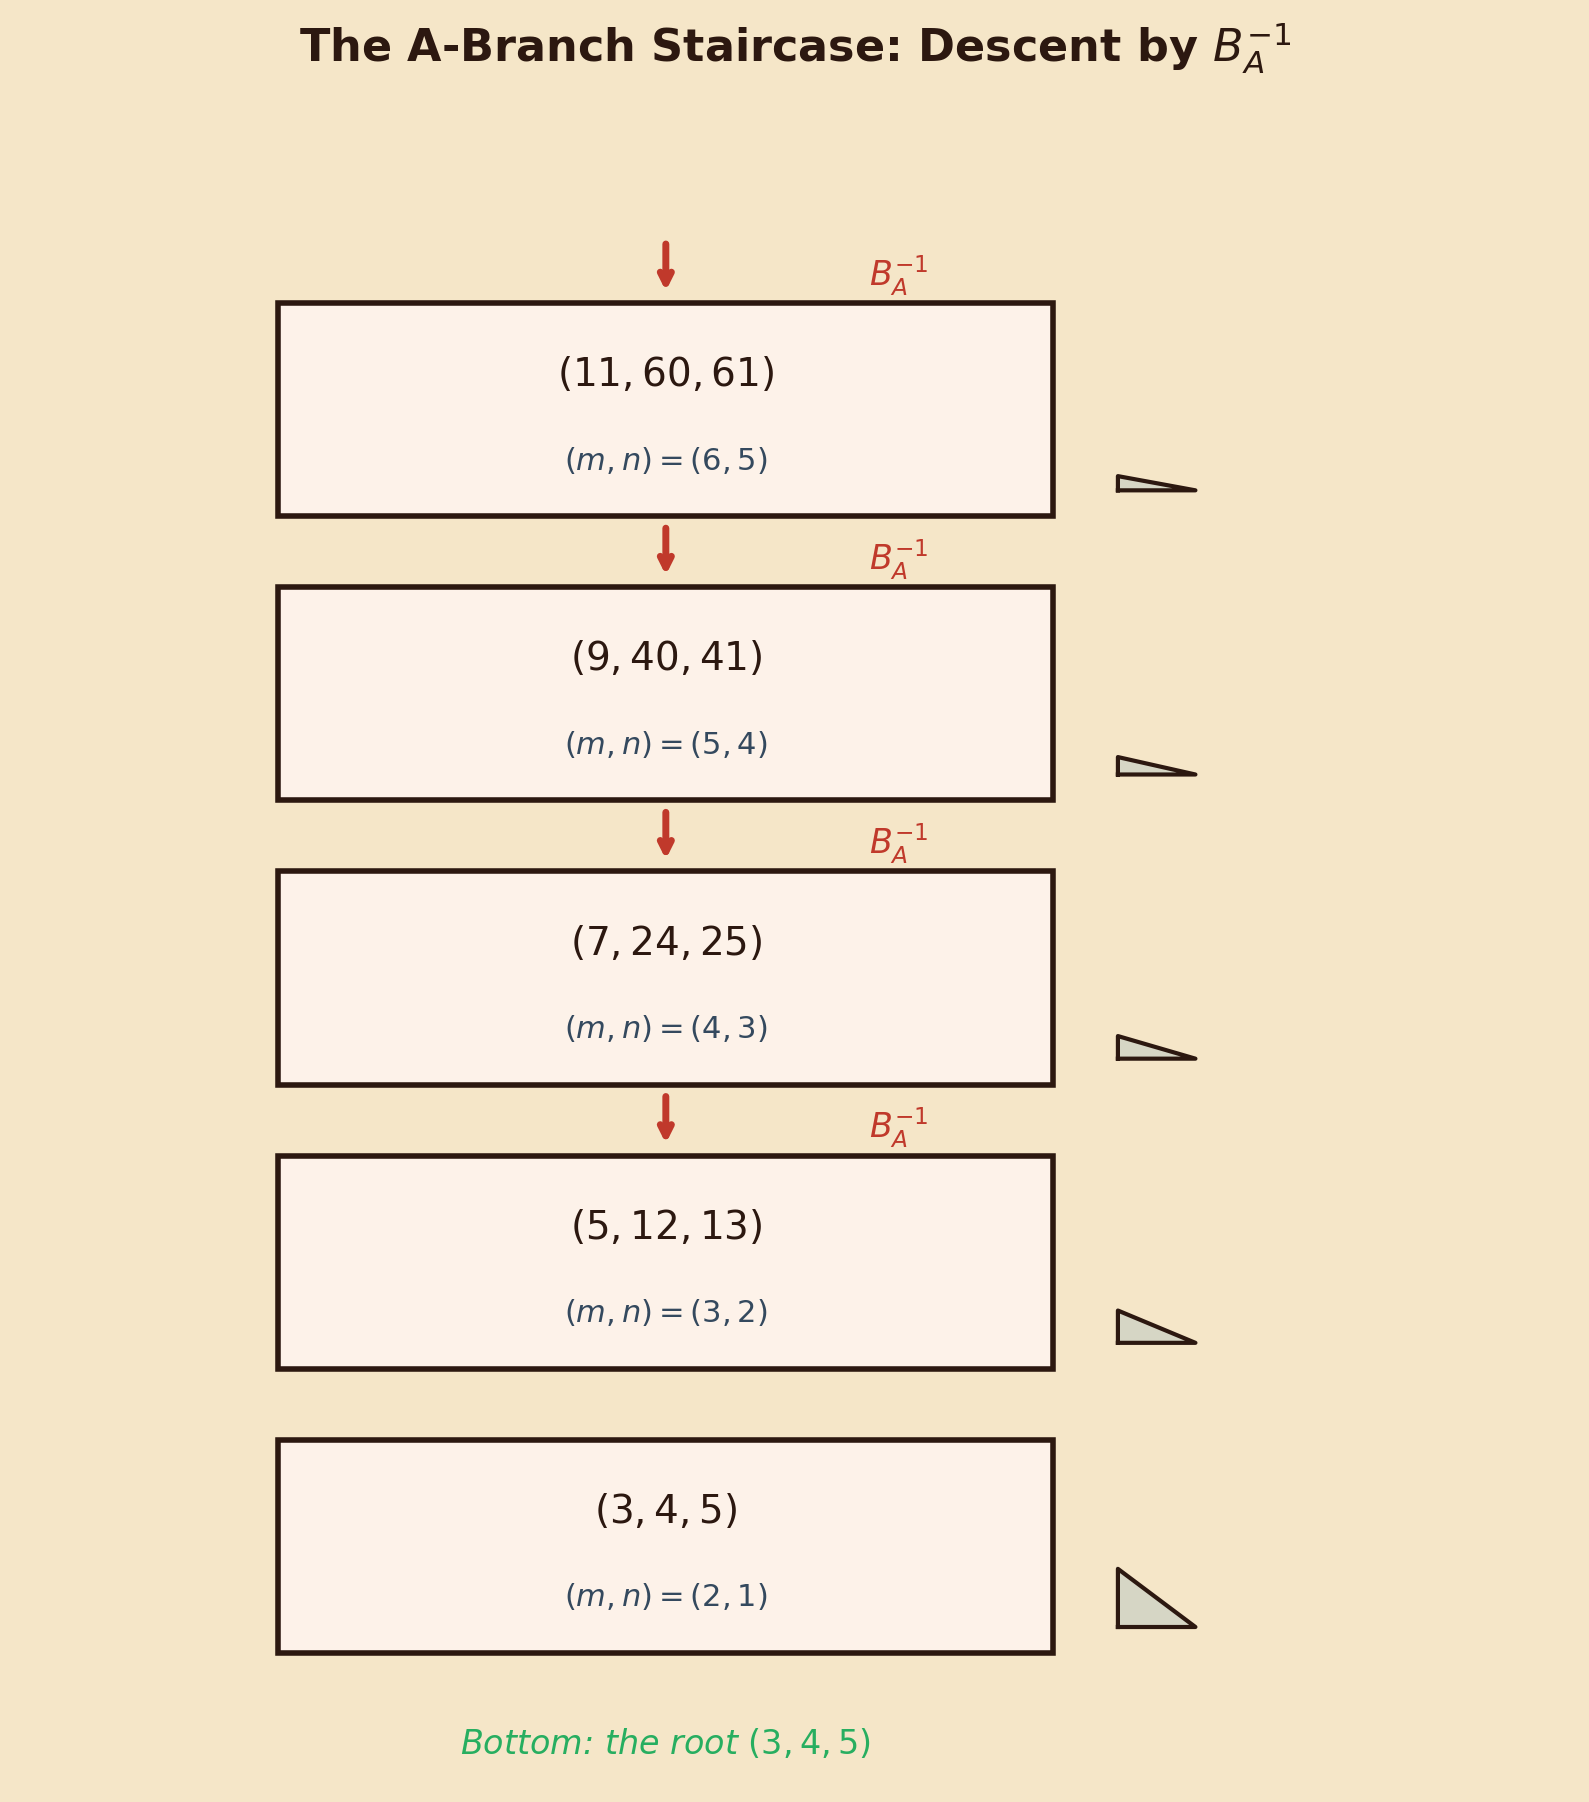
\includegraphics[width=0.85\textwidth]{Chapter5/images/fig11_a_staircase.png}
\caption{}
\end{figure}
A vertical staircase drawn in side view (like an architectural cross-section), each step labeled with a Pythagorean triple. At the bottom: \((3, 4, 5)\) with label \((m,n) = (2,1)\). Above it: \((5, 12, 13)\) with \((3,2)\). Then \((7, 24, 25)\) with \((4,3)\). Then \((9, 40, 41)\) with \((5,4)\). Arrows point downward along the staircase, each labeled ``\(B_A^{-1}\).'' The staircase is clean and regular --- no branching, no choices. Beside each step, the triple is also inscribed inside a small right triangle drawn to relative scale.{]}

The staircase is a \emph{deterministic descent}: from any triple with consecutive parameters, there is exactly one path to the root, and it uses only the \(A\)-branch. No choices, no backtracking, no guessing. The path from a triple back to \((3, 4, 5)\) is unique, and for the consecutive-parameter family, it is always a straight line of \(A\)-steps.

This has a lovely algorithmic interpretation. Given a triple with consecutive parameters, you can determine its ``depth'' in the Berggren tree instantly: it is simply \(m - 2\), the number of \(A^{-1}\) steps needed to reach the root. The triple \((9, 40, 41)\) has depth \(5 - 2 = 3\); the triple \((99, 4900, 4901)\) (from \(m = 50, n = 49\)) has depth 48.

\bigskip\noindent\rule{\linewidth}{0.4pt}\bigskip

\section{The Pell Staircase Along the B-Branch}
Now follow the \(B\)-branch of the tree --- always choosing \(B\), never \(A\) or \(C\) --- and watch the hypotenuses:

\[5, \quad 29, \quad 169, \quad 985, \quad 5741, \quad \ldots\]

Do you see the pattern? Each term is six times the previous one, minus the one before that:

\[c_0 = 5, \qquad c_1 = 29, \qquad c_{n+2} = 6\,c_{n+1} - c_n.\]

Verify: \(c_2 = 6 \times 29 - 5 = 174 - 5 = 169\). And \(169 = 13^2\) --- a perfect square! That is a delightful surprise. Continuing: \(c_3 = 6 \times 169 - 29 = 1014 - 29 = 985\). \(c_4 = 6 \times 985 - 169 = 5910 - 169 = 5741\).

The legs obey the same recurrence:

\[a_0 = 3,\quad a_1 = 21,\quad a_{n+2} = 6a_{n+1} - a_n,\] \[b_0 = 4,\quad b_1 = 20,\quad b_{n+2} = 6b_{n+1} - b_n.\]

Why does the magic number \(6\) appear? The answer lies in the eigenvalues of \(B_B\). The characteristic polynomial of the \(2 \times 2\) block that governs the recurrence satisfies

\[\lambda^2 - 6\lambda + 1 = 0,\]

yielding eigenvalues \(\lambda = 3 \pm 2\sqrt{2}\).

And here is the connection that sends a shiver down the spine of any number theorist: \(3 + 2\sqrt{2} = (1 + \sqrt{2})^2\), and \(1 + \sqrt{2}\) is the \emph{fundamental solution} of the Pell equation

\[x^2 - 2y^2 = 1.\]

The Pell equation! One of the oldest and most celebrated equations in all of number theory, with a history stretching back to Archimedes' cattle problem, through Brouncker's ingenious solution, Euler's famous misattribution (John Pell had nothing to do with it), and Lagrange's general proof that solutions always exist for non-square \(d\).

The convergents of the continued fraction for \(\sqrt{2}\) are

\[\frac{1}{1}, \quad \frac{3}{2}, \quad \frac{7}{5}, \quad \frac{17}{12}, \quad \frac{41}{29}, \quad \ldots\]

Notice \(29\) --- the hypotenuse of the first \(B\)-child \((21, 20, 29)\) --- appearing as the denominator of a convergent. The numerators and denominators of these convergents satisfy the very same recurrence \(x_{n+2} = 2x_{n+1} + x_{n-1}\), which, after a change of variables, yields our \(c_{n+2} = 6c_{n+1} - c_n\).

The \(B\)-branch of the Berggren tree is secretly tracing the solutions of a Pell equation. Each step along the branch produces the next Pell approximant to \(\sqrt{2}\), encoded as a Pythagorean triple. The ratios \(b_n / a_n\) converge to \(1\) and \(c_n / b_n\) converges to a value related to \(\sqrt{2}\) --- the branch is simultaneously generating right triangles and solving a Diophantine equation of a completely different type.


\begin{figure}[htbp]
\centering
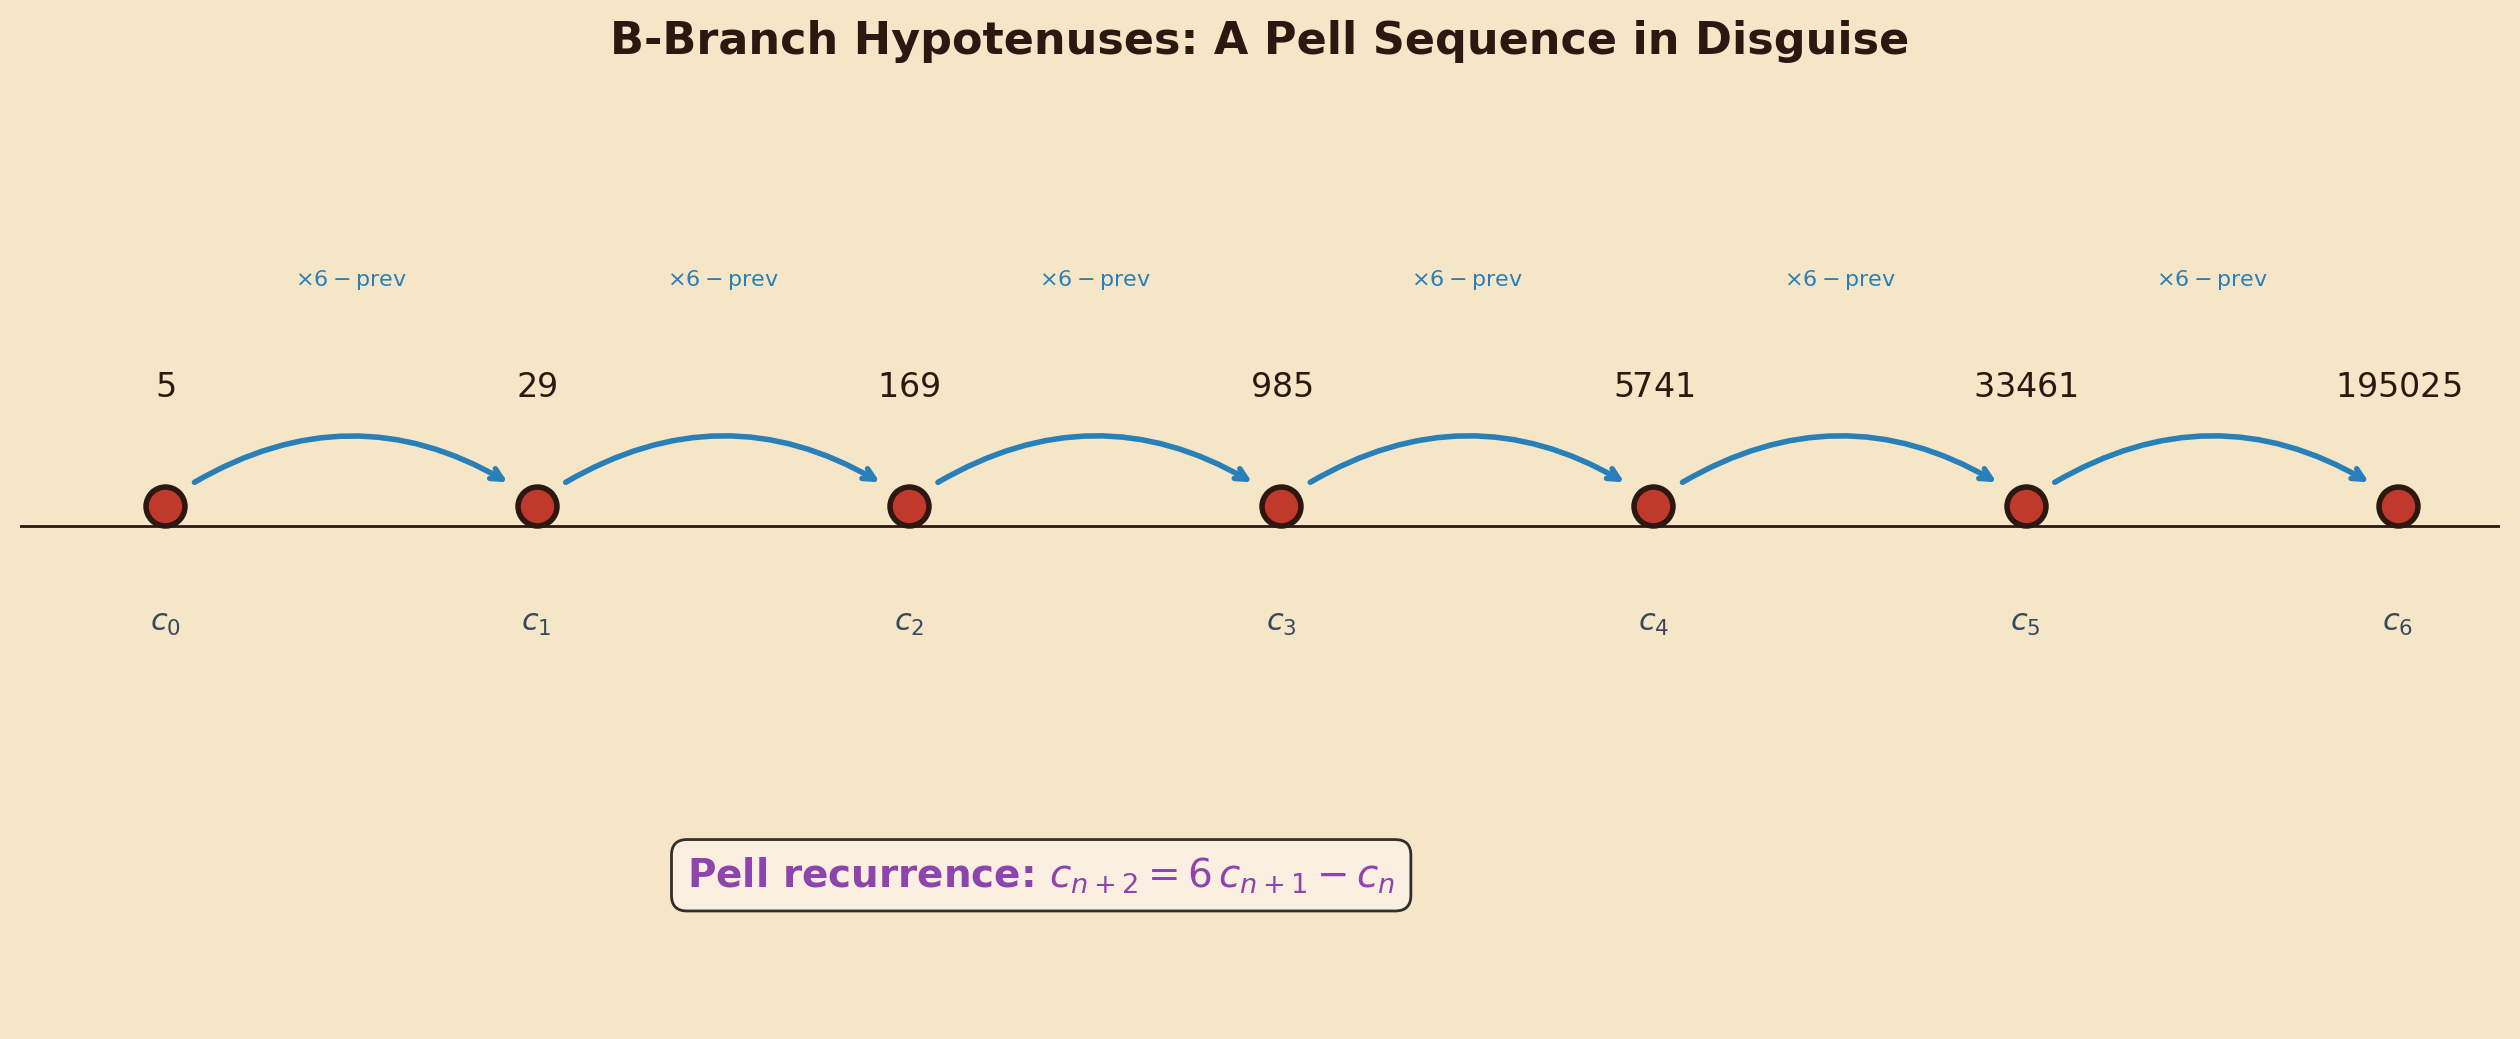
\includegraphics[width=0.85\textwidth]{Chapter5/images/fig12_pell_number_line.png}
\caption{}
\end{figure}
A number line (logarithmic scale) showing the B-branch hypotenuses \(5, 29, 169, 985, 5741\) at exponentially increasing intervals. Curved arrows between consecutive terms, labeled ``\(\times 6 - \text{prev}\).'' Below the number line, a spiral evokes the continued fraction convergents of \(\sqrt{2}\), with the same numbers appearing as denominators of the convergents: \(\ldots, 5, 29, 169, \ldots\){]}


\begin{figure}[htbp]
\centering
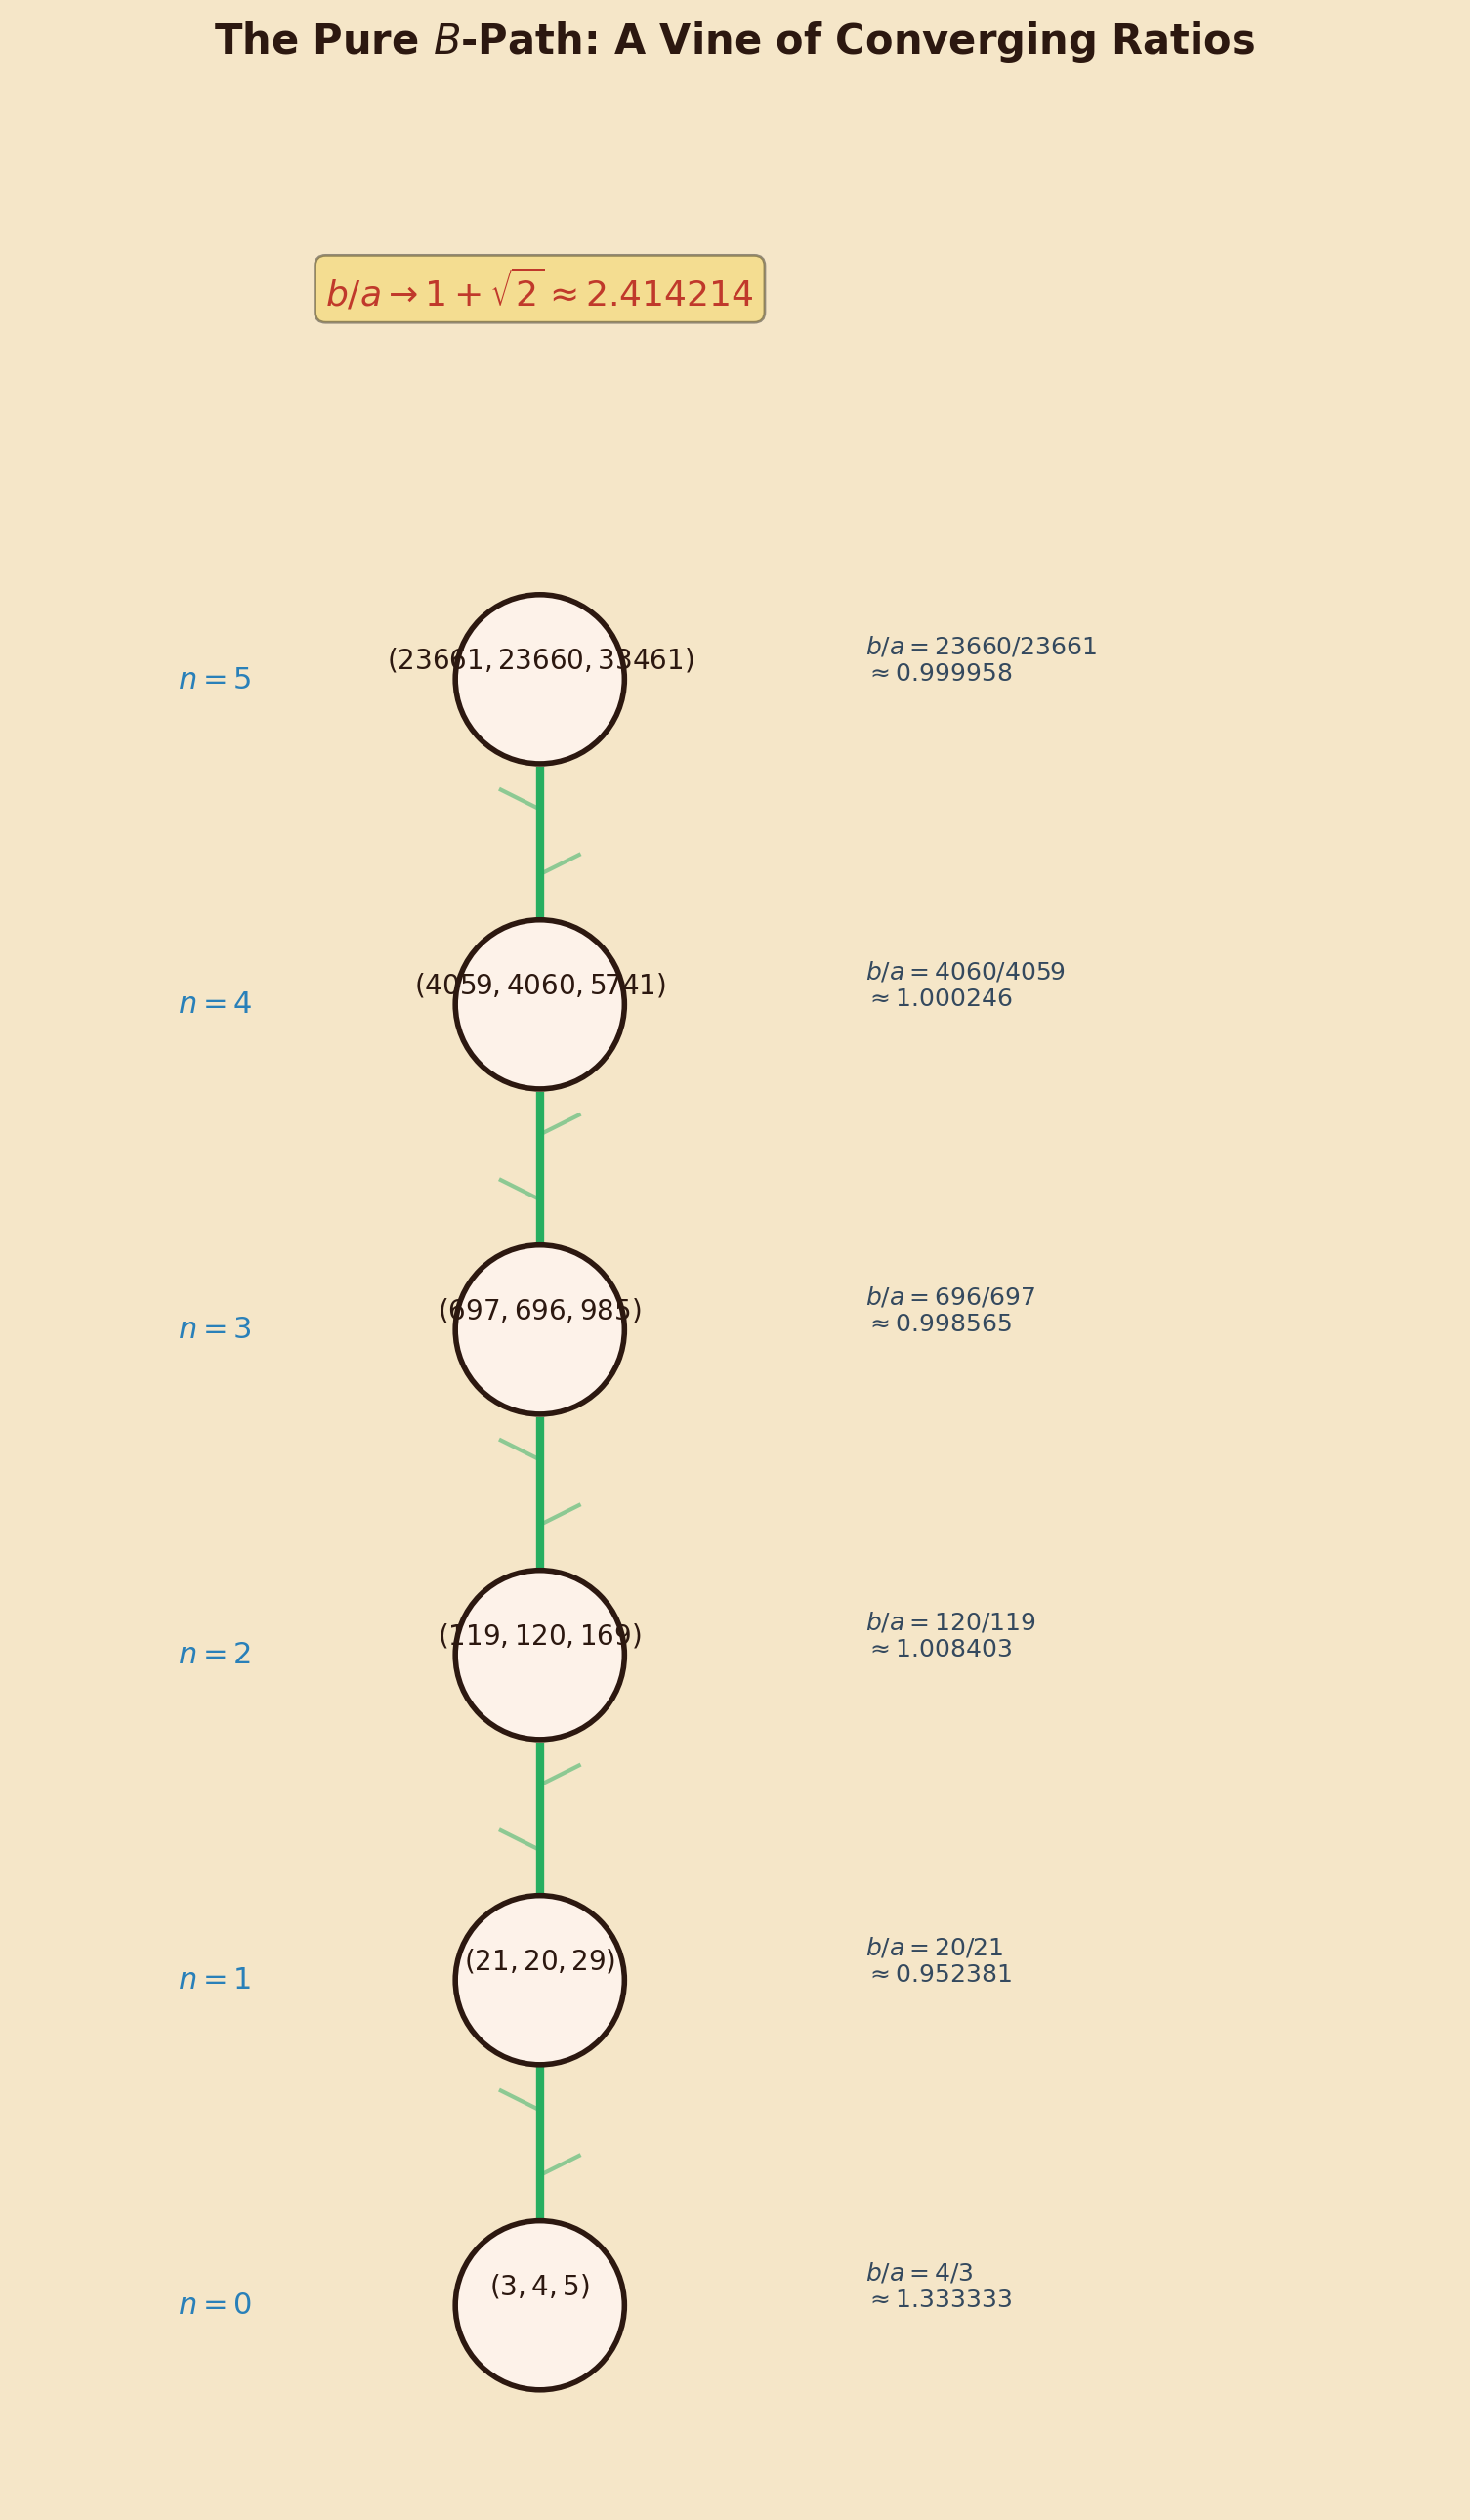
\includegraphics[width=0.85\textwidth]{Chapter5/images/fig13_b_branch_vine.png}
\caption{}
\end{figure}
A single vertical ``branch'' of the Berggren tree --- the pure \(B\)-path, rendered as a vine growing upward. At each node (rendered as a leaf), the full triple \((a_n, b_n, c_n)\) is listed. Beside each node, the ratio \(b_n / a_n\) is computed to several decimal places, showing convergence. The vine should have an organic quality, evoking growth and regularity in tandem.{]}

\bigskip\noindent\rule{\linewidth}{0.4pt}\bigskip

\section{The Grand Unification --- Eight Theorems and the View from Above}
We have now assembled all the pieces. Let us step back and see the whole mosaic.

Eight theorems, each proved with nothing beyond algebra and induction, reveal one of the most beautiful correspondences in all of mathematics. Here they are, gathered into a single panoramic view:

\textbf{1. Lorentz Preservation.} Each Berggren matrix \(M\) satisfies \(M^\top \eta\, M = \eta\), where \(\eta = \mathrm{diag}(1, 1, -1)\). The matrices are integer Lorentz transformations: discrete symmetries of spacetime geometry.

\textbf{2. Pythagorean Preservation.} If \((a, b, c)\) satisfies \(a^2 + b^2 = c^2\), then so does \(M(a, b, c)\) for each \(M \in \{B_A, B_B, B_C\}\). The Pythagorean property is hereditary.

\textbf{3. Tree Soundness.} Every node of the Berggren tree satisfies \(a^2 + b^2 = c^2\). By induction on the tree, the guarantee is absolute and eternal.

\textbf{4. The Factoring Identity.} For any Pythagorean triple, \((c - b)(c + b) = a^2\) --- a bridge from geometry to number theory, and a primitive ancestor of modern factoring algorithms.

\textbf{5. Euclid's Parametrization.} The identity \((m^2 - n^2)^2 + (2mn)^2 = (m^2 + n^2)^2\) holds for all integers --- a universal machine for manufacturing Pythagorean triples.

\textbf{6. Pell Recurrence.} The \(B\)-branch hypotenuses satisfy \(c_{n+2} = 6c_{n+1} - c_n\), tracing the solutions of \(x^2 - 2y^2 = 1\) through the tree.

\textbf{7. A-Branch Descent.} Triples with consecutive Euclid parameters \((m, m-1)\) descend to the root via pure \(B_A^{-1}\) steps --- a deterministic staircase.

\textbf{8. Determinants.} \(\det(B_A) = 1\), \(\det(B_B) = -1\), \(\det(B_C) = 1\). Two rotations and one reflection: the tree's branches have distinct geometric characters.

Surrounding these eight results is the Brahmagupta--Fibonacci identity,

\[(a_1^2 + b_1^2)(a_2^2 + b_2^2) = (a_1 a_2 - b_1 b_2)^2 + (a_1 b_2 + b_1 a_2)^2,\]

the capstone that connects the multiplicative structure of sums of squares to Gaussian integer norms --- \(|z_1 z_2|^2 = |z_1|^2 |z_2|^2\) --- and explains why the factoring identity has teeth: if \(N^2\) is a sum of two squares in multiple ways, each representation gives a shot at a factor.

The philosophical payoff is worth savoring. These eight theorems require no advanced machinery. No complex analysis, no algebraic geometry, no abstract algebra beyond the definition of a group. The tools are:

\begin{itemize}
\tightlist
\item
  Matrix multiplication.
\item
  The expansion of \((x + y)^2\).
\item
  Mathematical induction (on trees).
\item
  The observation that \(c^2 - b^2 = (c - b)(c + b)\).
\end{itemize}

Four tools. Eight theorems. And they reveal a web of connections between:

\begin{itemize}
\tightlist
\item
  \textbf{Ancient Greek geometry} (Euclid's parametrization, the Pythagorean theorem itself).
\item
  \textbf{7th-century Indian algebra} (Brahmagupta's identity).
\item
  \textbf{19th-century number theory} (Pell equations, continued fractions).
\item
  \textbf{20th-century physics} (the Lorentz group, Minkowski spacetime).
\item
  \textbf{21st-century cryptography} (integer factoring as the foundation of public-key security).
\end{itemize}

Five civilizations, five centuries of mathematical effort, one equation: \(a^2 + b^2 = c^2\).


\begin{figure}[htbp]
\centering
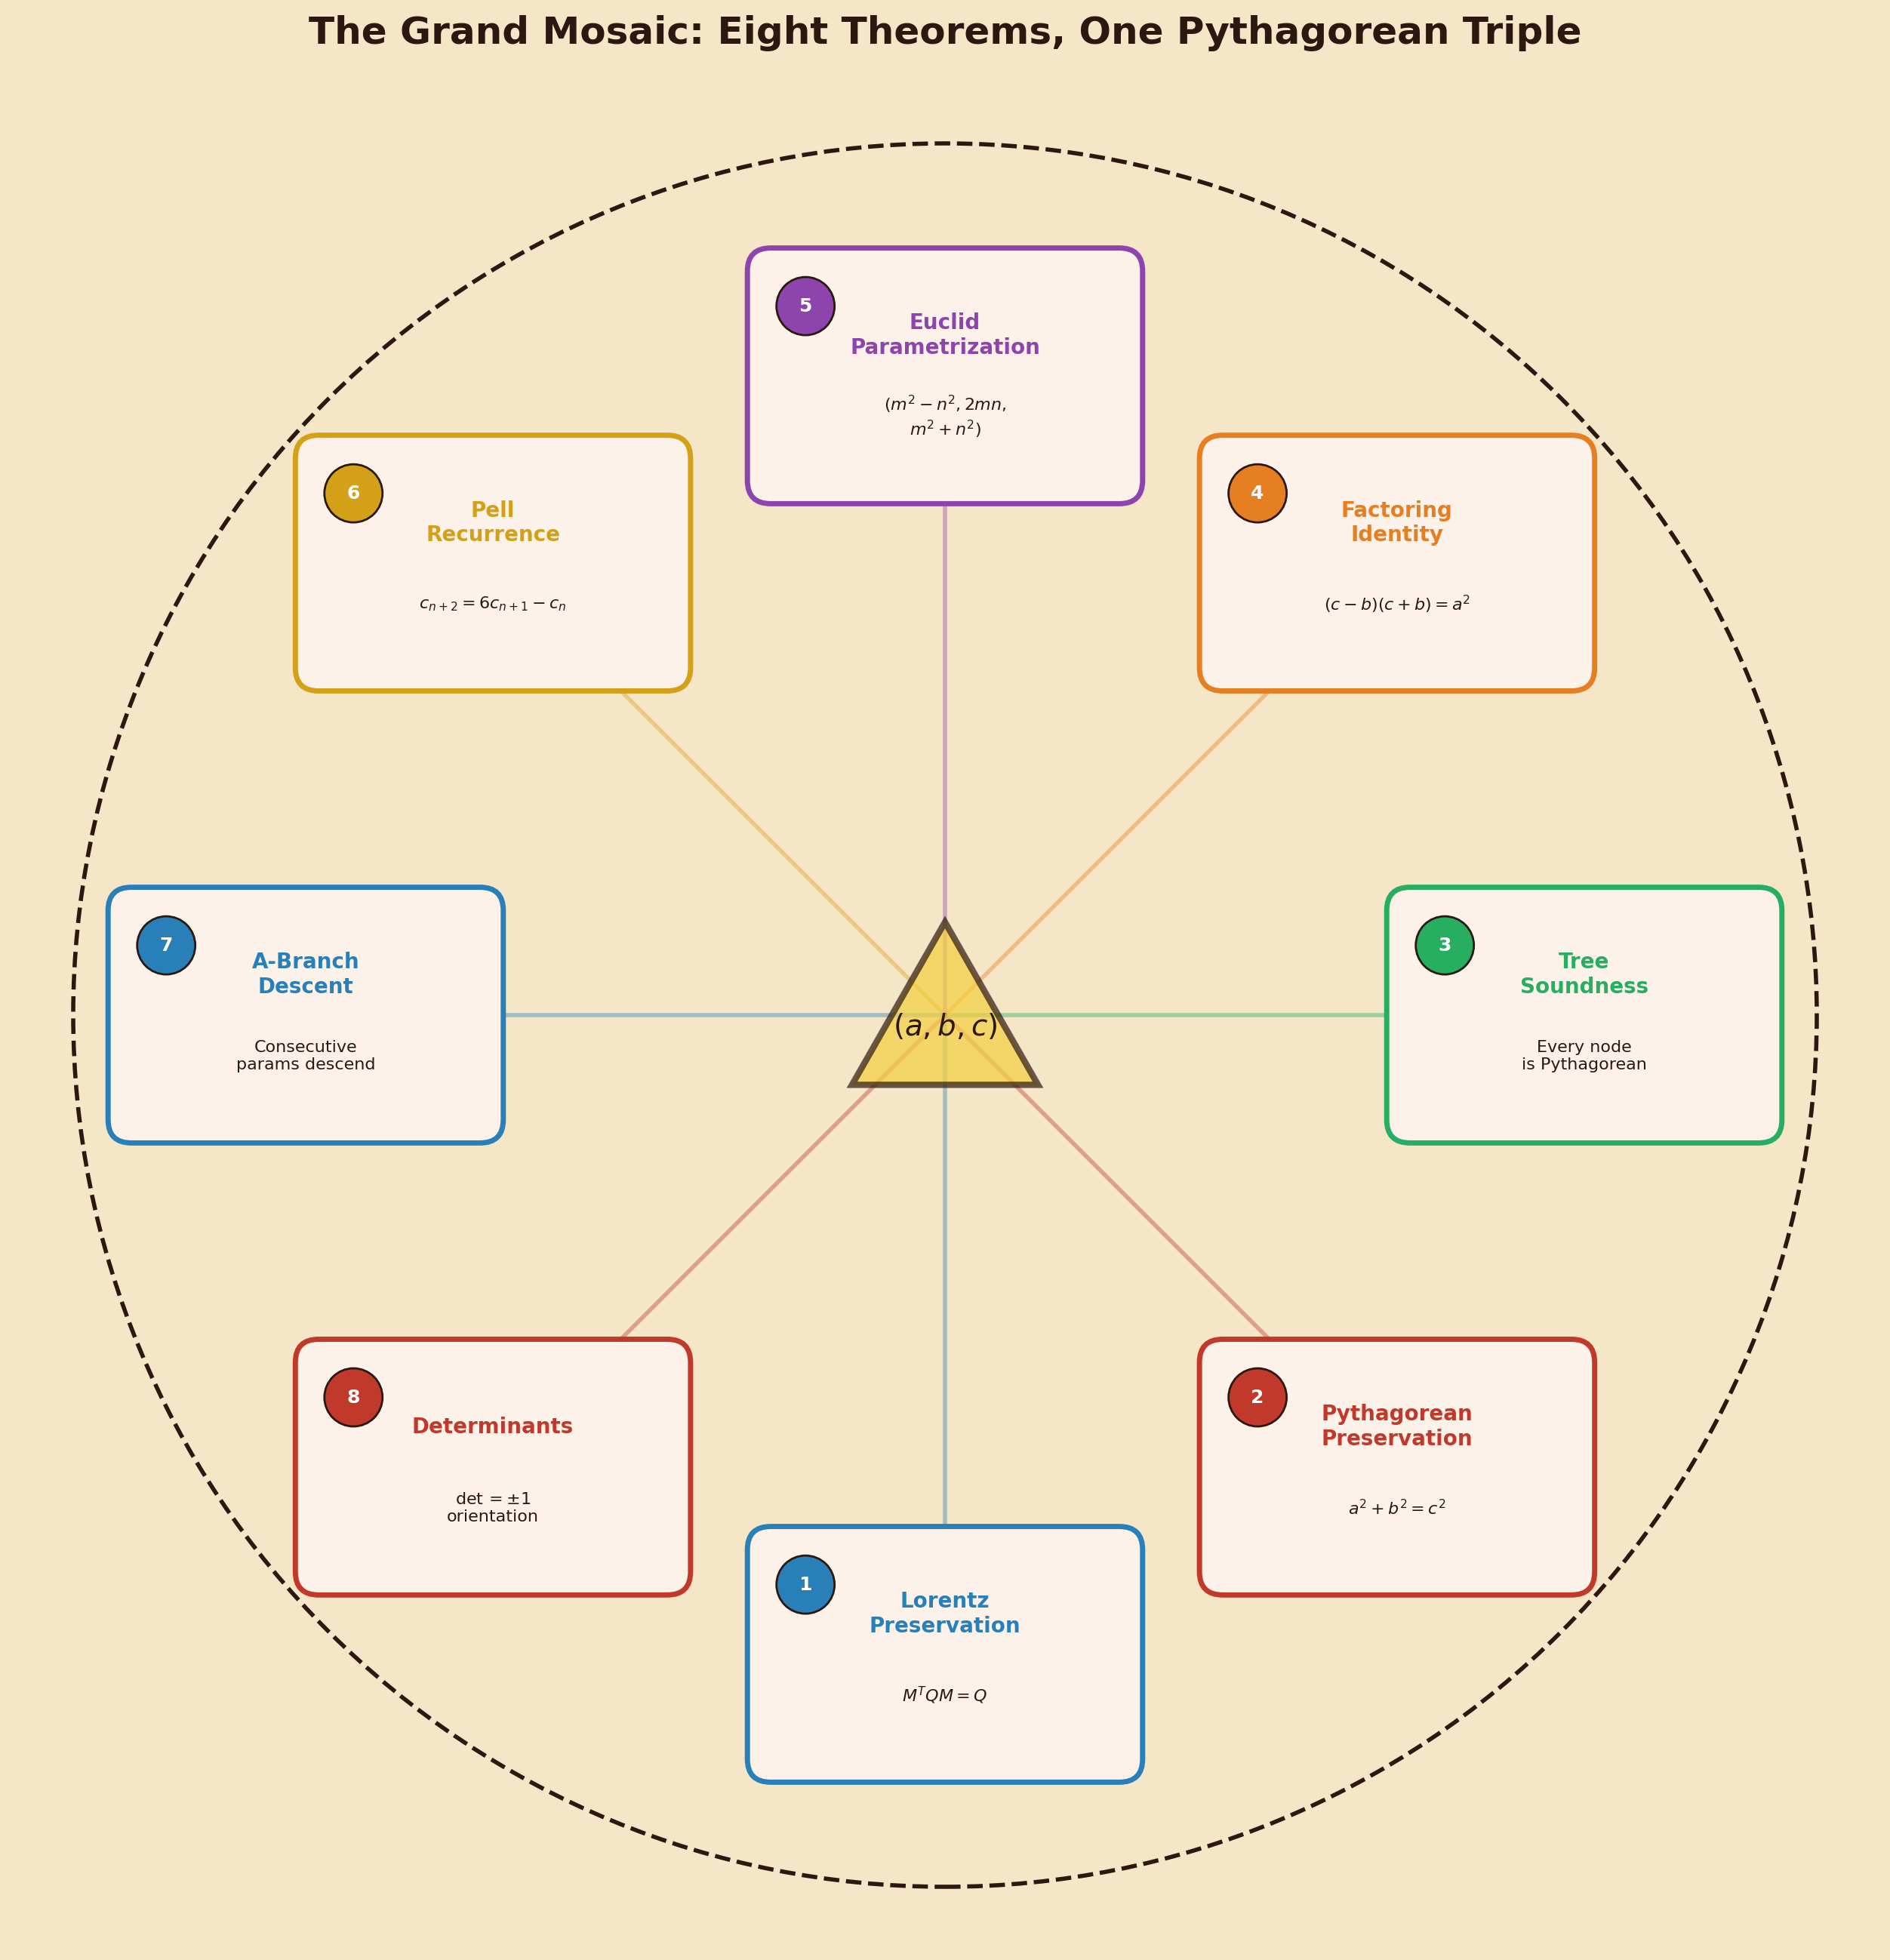
\includegraphics[width=0.85\textwidth]{Chapter5/images/fig14_grand_mosaic.png}
\caption{}
\end{figure}
A large, ornate diagram --- the ``Grand Mosaic.'' At the center, a Pythagorean triple \((a, b, c)\) inscribed in a glowing right triangle. Radiating outward in eight directions, like the points of a compass rose, labeled paths lead to eight icons representing the eight theorems: a \(3 \times 3\) matrix for Lorentz Preservation; a triangle with a checkmark for Pythagorean Preservation; a branching tree for Soundness; a pair of scissors cutting a number for the Factoring Identity; the letters \(m, n\) for Euclid; a spiral for Pell; a descending staircase for A-Descent; and a hand mirror for Determinants. The whole composition evokes a Renaissance-era mathematical broadsheet --- ornamental borders, classical typography, a sense of timeless authority.{]}


\begin{figure}[htbp]
\centering
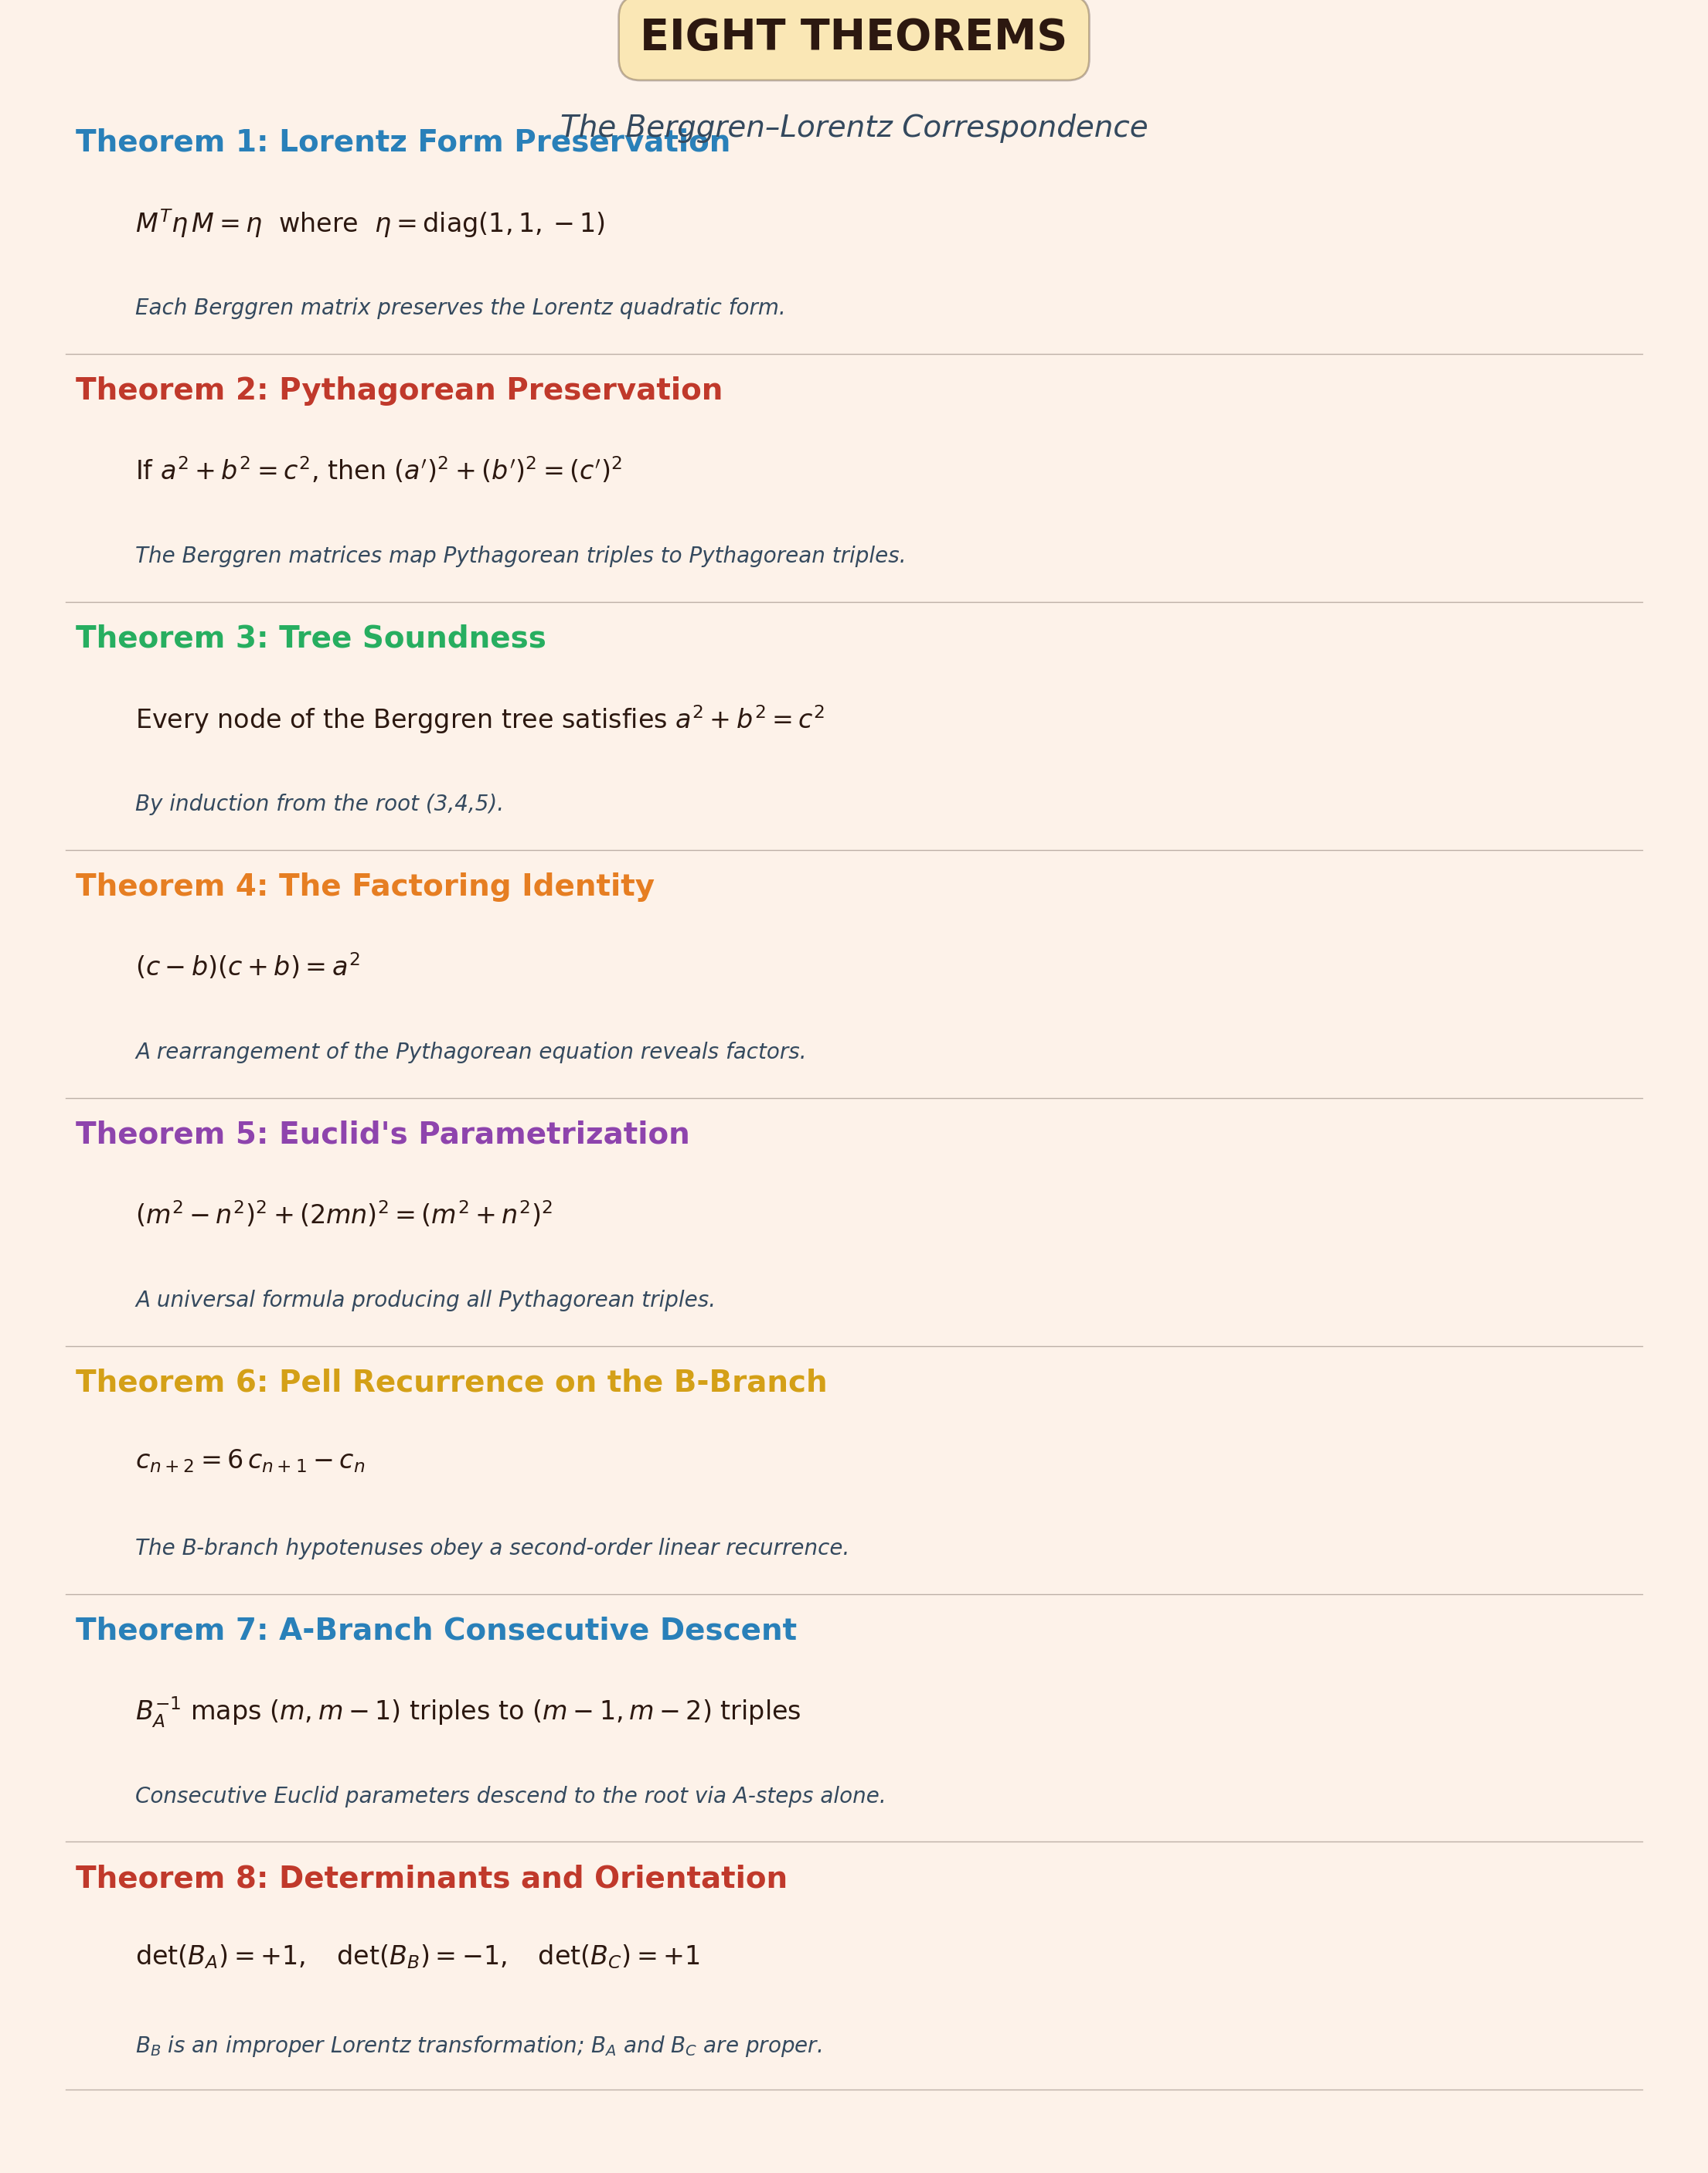
\includegraphics[width=0.85\textwidth]{Chapter5/images/fig15_cheat_sheet.png}
\caption{}
\end{figure}
A full-page ``cheat sheet'' showing all eight theorem statements in clean mathematical typesetting, each numbered and titled. The layout is two columns, with generous whitespace and classical serif fonts. Each theorem's statement is concise --- one or two lines of displayed mathematics --- with a one-sentence plain-English summary beneath. The aesthetic evokes a page from Euclid's \emph{Elements}: clean, authoritative, suitable for framing.{]}

I will leave you with a puzzle to carry into the next chapter. Suppose you want to factor the number \(N = 1{,}000{,}003\). Can you find a Pythagorean triple with \(a = N\)? If so, the factoring identity hands you \((c - b)\) and \((c + b)\), and \(\gcd(N, c - b)\) may be a nontrivial factor. The task is not as hopeless as it sounds: the Berggren tree provides a systematic way to search for triples with any given leg, and the search is guided by the very symmetries of the tree.

Try it --- and see if the factors emerge.

\bigskip\noindent\rule{\linewidth}{0.4pt}\bigskip

\emph{In the next chapter, we will reverse the telescope: instead of looking outward from the tree's root to its infinitely many leaves, we will look inward, asking how the tree's branching structure encodes the continued fraction expansion of \(\sqrt{2}\) and the geometry of the hyperbolic plane. The tree, it will emerge, is not merely a list dressed as a graph. It is a tessellation --- a tiling of non-Euclidean space by ideal triangles, with each tile corresponding to a primitive Pythagorean triple. The tree knew it was a spacetime all along.}
